% \documentclass{article}
% \documentclass[twocolumn]{IEEEtran}
\documentclass{llncs}

% Proof already defined in llncs so I am 
% relaxing it for amsthm
\let\proof\relax
\let\endproof\relax

\usepackage{hyperref}

\usepackage{algorithm}
\usepackage[noend]{algpseudocode}

\RequirePackage{amssymb, mathptm}
\usepackage{amsbsy}
\usepackage{amsthm}
\usepackage{graphicx}
\usepackage{helvet}
\usepackage{enumerate}
\usepackage{amsmath}
\usepackage{amsfonts}
\usepackage{graphicx}
\usepackage{multirow}
\usepackage{subfig}
\usepackage{comment}
\usepackage{cases}
\usepackage{xcolor}
\usepackage{epstopdf}
\usepackage[normalem]{ulem}
\usepackage{diagbox}
\usepackage{bm}
\usepackage{hhline}
\usepackage{caption}


% \bibliographystyle{plain}
\newcommand{\B}{{\mathbb{B}}}
\newcommand{\Z}{{\mathbb{Z}}}
\newcommand{\R}{{\mathbb{R}}}
\newcommand{\Q}{{\mathbb{Q}}}
\newcommand{\N}{{\mathbb{N}}}
\newcommand{\C}{{\mathbb{C}}}
\newcommand{\Zn}{{\mathbb{Z}}_{n}}
\newcommand{\Zp}{{\mathbb{Z}}_{p}}
\newcommand{\F}{{\mathbb{F}}}
\newcommand{\FF}{{\mathcal{F}}}
\newcommand{\Fbar}{{\overline{\mathbb{F}}}}
\newcommand{\Fq}{{\mathbb{F}}_{q}}
\newcommand{\Fqbar}{{\overline{{\mathbb{F}}_q}}}
\newcommand{\Fkk}{{\mathbb{F}}_{2^k}}
\newcommand{\Zkk}{{\mathbb{Z}}_{2^k}}
\newcommand{\Fkkx}[1][x]{\ensuremath{\mathbb{F}}_{2^k}[#1]\xspace}
\newcommand{\Grobner}{Gr\"{o}bner\xspace}
\newcommand{\bi}{\begin{itemize}}
\newcommand{\ei}{\end{itemize}}

\newcommand{\idealj}{{J = \langle f_1, \dots, f_s\rangle}}
\newcommand{\idealg}{{J = \langle g_1, \dots, g_t\rangle}}
\newcommand{\vfqj}{{V_{\Fq}(J)}}
\newcommand{\vfkkj}{{V_{\Fkk}(J)}}

%%% Added by Utkarsh %%%
\newcommand{\Va}{{V_A}}
\newcommand{\Vb}{{V_B}}
\newcommand{\Vc}{{V_C}}
\newcommand{\Vbc}{{V_{B,C}}}
\newcommand{\Vabc}{{V_{A,B,C}}}
\newcommand{\Vac}{{V_{A,C}}}
\newcommand{\w}{\wedge}

%%%%%%%%%%%%%%%%%%%%%%%%

\newcommand{\blu}{\color{blue}}
% \newcommand{\Grobner}{Gr\"{o}bner\xspace}
\newcommand{\fqring}{\Fq[x_1,\dots,x_n]}


% \newtheoremstyle{mystyle}
%   {\topsep}   % ABOVESPACE
%   {\topsep}   % BELOWSPACE
%   {\itshape}  % BODYFONT
%   {0pt}       % INDENT (empty value is the same as 0pt)
%   {\bf} % HEADFONT
%   {.}         % HEADPUNCT
%   {5pt plus 1pt minus 1pt} % HEADSPACE
%   {}          % CUSTOM-HEAD-SPEC

% \theoremstyle{plain}
\theoremstyle{definition}
% \theoremstyle{remark}
% \theoremstyle{mystyle}

\newtheorem{Algorithm}{Algorithm}[section]

\newtheorem{Definition}{Definition}[section]
\numberwithin{Definition}{section}

\newtheorem{Example}{Example}[section]
\numberwithin{Example}{section}

\newtheorem{Proposition}{Proposition}[section]

\newtheorem{Lemma}{Lemma}[section]
\numberwithin{Lemma}{section}

\newtheorem{Theorem}{Theorem}[section]
\numberwithin{Theorem}{section}

\newtheorem{Corollary}{Corollary}[section]
\newtheorem{Conjecture}{Conjecture}[section]
\newtheorem{Problem}{Problem}[section]
\newtheorem{Notation}{Notation}[section]
\newtheorem{Setup}{Problem Setup}[section]

\begin{document}

\title{Craig Interpolants in Finite Fields using Algebraic Geometry:
  Theory and Algorithms\thanks{This research is funded in part by the
    US National Science Foundation grants CCF-1619370 and
    CCF-1320385.}} 

\author{Utkarsh Gupta$^1$ \and Irina Ilioaea$^2$ \and Priyank Kalla$^1$ \and Florian Enescu$^2$\\
$^1$Electrical and Computer Engineering, University of Utah, Salt Lake City UT, USA \\
$^2$Mathematics and Statistics, Georgia State University, Atlanta GA, USA
}

\institute{}
\maketitle

\thispagestyle{plain}
\pagestyle{plain}



\begin{abstract}

Resolving an unknown component is a fundamental problem encountered in
post-verification debugging and automatic correction of digital
circuits. Contemporary techniques rely on iterative/incremental
application of SAT solving and Craig interpolation to realize the
functionality of (or resolve) the unknown components. While these
techniques have achieved some success for control-dominated
applications (random logic circuits), they are infeasible in resolving
the unknown components in arithmetic circuits. This paper describes an
algebraic approach to resolve the functionality of an unknown
component in a finite field arithmetic circuit so that the circuit
implementation matches a given specification. Starting from an
equivalence checking setup modeled as a polynomial ideal
membership test in commutative algebra, we formulate the problem of
resolving the unknown component as a quantification procedure. Using
the \Grobner basis algorithm, we derive an approach to identify the
function implemented by the unknown component. We go on to pose the
problem as a synthesis challenge and explore the space of polynomial
functions for the unknown component by analyzing quotients of
ideals. As \Grobner basis algorithms exhibit high computational
complexity, we exploit the circuit topology to improve our
algorithms. We can resolve the unknown components not just for
bit-level circuit implementations, but also in cases where the
abstraction hierarchy is given at the level of (bit-vector)
words. Experiments performed over various finite field arithmetic
circuits demonstrate the efficacy and superiority of our approach as
compared to conventional techniques.

  % Resolving an unknown component is a fundamental problem encountered
  % in logic synthesis for engineering change orders, post-verification
  % debugging and automatic correction of digital circuits. Contemporary
  % techniques rely on the iterative/incremental application of SAT solving
  % and Craig interpolation to realize the functionality of (or resolve)
  % the unknown components. While these techniques have achieved some
  % success for control-dominated applications (random logic circuits),
  % they are infeasible in resolving the unknown components in
  % arithmetic circuits. This paper describes an algebraic approach to
  % resolve the functionality of an unknown component in an arithmetic
  % circuit so that the circuit implementation matches a given
  % specification. Our approach is formulated as a polynomial ideal
  % membership test. We go on to pose the problem as a synthesis
  % challenge and explore the solution space of the unknown component
  % using concepts from the quotient of ideals. We propose a \Grobner basis 
  % based algorithm for a systematic, goal driven search for
  % implementable solutions. The paper presents results on some
  % experiments performed over various finite field arithmetic circuits
  % to compare the efficiency of our approach against recent methods.   


% Automatic bug correction is a tedious and resource intensive process. 
%% Automatic correction of unknown components in a given circuit is a
%% resource intensive process. Recent developments in realizing the
%% functionality implemented by these unknown gates rely on incremental
%% SAT solving. Despite using state-of-the-art SAT solvers, these
%% approaches fail to verify multipliers beyond 12-bits and hence are
%% infeasible in a practical setting. The current formal datapath
%% verification methods which utilize symbolic computer algebra concepts,
%% rely heavily on textbook structure of the circuits to realize an
%% unknown component, and hence are not scalable. These approaches model
%% circuit as a set of polynomials over integer rings, and use function
%% extraction, simulation, and term rewriting using coefficient
%% computation to arrive at a solution. The approach is not complete in
%% the sense that the procedure cannot be extended to random logic
%% circuits and finite field circuits due to ambiguities in coefficient
%% computation. The approach also fails to verify circuits when redundant
%% gates are introduced in the design. To overcome all these limitations,
%% this paper describes a formal approach using finite field theory to
%% automatically realize the function implemented by an unknown
%% component, and verify the same. The paper introduces theory on
%% resolving a single unknown component using ideal membership testing
%% and \Grobner basis based reduction. We go onto pose the problem as a
%% synthesis challenge and extend the solution space of the unknown
%% component using concepts from quotient of ideals. Since the solution
%% space is not unique, we will also discuss a systematic, goal driven
%% search for simple implementable solutions. The paper presents results
%% on some preliminary experiments performed over various arithmetic
%% circuits to compare efficiency of our approach against recent methods.  
\end{abstract}

\section{Introduction}

Craig interpolation is a method to construct and refine abstractions
of functions. It finds application in formal verification of hardware
designs and software programs, in logic synthesis of Boolean
functions, and also as a tool in proof complexity theory. It is a
logical tool to extract concise explanations for the infeasibility of
a mutually inconsistent set of statements. Craig
\cite{craig-interpolate} showed that for a valid implication $A
\implies B$, where $A, B$ are first order formulae containing no free
variables, there is a formula $I$ such that $A \implies I$, $I
\implies B$ and the non-logical symbols of $I$ appear in both $A$ and
$B$. The formula $I$ is called the {\it Craig interpolant}, or
interpolant for short. As  
propositional logic also admits Craig interpolation, the formal
verification community has extensively investigated interpolants and
their computation from resolution proofs of CNF-SAT problems. In the
propositional logic domain, the concept is stated with a slight
modification.  

\begin{Definition}\label{def:ci}
Let $(A, B)$ be a pair of CNF formulae (sets of clauses) such that $A
\w B$ is unsatisfiable. Then there exists a formula $I$ such that: (i)
$A\implies I$; (ii) $I \w B$ is unsatisfiable; and (iii) $I$ refers
only to the common variables of $A$ and $B$, i.e. $Var(I) \subseteq
Var(A) \cap Var(B)$. The formula $I$ is called the {\bf interpolant}
of $(A,B)$. 
\end{Definition}

Given the pair $(A, B)$ and their refutation proof, a procedure called
the {\it interpolation system} constructs the interpolant in linear
time and space in the size of the proof \cite{McMillan:CAV03}. As the
abilities of SAT solvers for proof refutation have improved,
interpolants have been exploited as abstractions in various problems
that can be formulated as unsatisfiable instances, e.g. model checking
\cite{McMillan:CAV03}, logic synthesis \cite{roland:bidecomp},
etc. Their use as abstractions have also been replicated in other
(combinations of) theories \cite{McMillan:TACAS04}
\cite{Kapur:SIGSOFT06} \cite{Cimatti:TACAS08} \cite{Griggio:FMCAD11},
etc.  
%These concepts have been applied to various problems in
%automated reasoning. 
%; {\it e.g.} for the theory of linear
%inequality \cite{McMillan:TACAS04}, data-type theories
%\cite{Kapur:SIGSOFT06}, Linear arithmetic and difference logic
%\cite{Cimatti:TACAS08}, Bit-vector theories \cite{Griggio:FMCAD11},
%among others.  


In this paper, we introduce the notion of {\it Craig interpolants in
polynomial algebra over finite fields} ($\Fq$) of $q$ elements, where
$q = p^k$ is a prime power. Given a mutually inconsistent pair of sets
of polynomials with coefficients from $\Fq$ that have no common zeros,
we show that Nullstellensatz over finite fields admits
interpolation. We represent the sets $A, B$ (from Def. \ref{def:ci}) as
{varieties of corresponding ideals}, and prove the existence of
an interpolant for the pair $(A,B)$. In this setting, {\it interpolants
correspond to varieties} -- subsets of the $n$-dimensional affine
space $\Fq^n$ -- and are represented by polynomial ideals, more
precisely, by a {\it Gr\"obner basis of corresponding ideals.}

Intuitively, it should be apparent that polynomial algebra over finite
fields would admit Craig interpolation (a first order theory over
$\Fq$ definitely admits quantifier elimination \cite{gao:qe-gf-gb}).
However, our literature search for interpolants and their computation
with polynomials in arbitrary finite fields did not reveal much prior
work in this area. %turned out to be unsuccessful. 
%There is a need for the theory and algorithms for
%interpolation in this domain. 
Recent years have witnessed
investigations in formal verification, abstraction and synthesis of
datapath circuits with $k$-bit operands, where the problems have been
modeled 
%using algebraic geometry 
over finite fields ($\Fkk$) \cite{pruss:tcad} \cite{xiaojun:hldvt2016}
or over finite integer rings ($\Zkk$) \cite{sivaram:todaes}. 
%Analogous to Boolean
%function decomposition, 
%there is also a need for polynomial (word-level) datapath synthesis
Interpolants can be exploited as abstractions of functions
($f:\Fkk\rightarrow\Fkk$) in this domain, and can make these
approaches practical. Motivated by the above needs, this paper
presents the theory of Craig interpolation in finite fields, and
describes algorithms to compute them.  


{\it Contributions:} Using the extensive machinery of algebraic
geometry in finite fields,
% -- including Nullstellensatz, projections of
%varieties, elimination and extension theory, set operations on ideals
%and varieties, etc. -- 
this paper makes the following contributions: 
1) Formally define the notion of interpolants in polynomial algebra
  over finite fields $\Fq$, and prove their existence in this domain.
2) Derive the relationship of interpolants with elimination ideals,
  and show how to compute them using Gr\"obner bases. 
3) Compute the {\it smallest} interpolant, i.e. the one
  contained in every other interpolant. Analogously, compute the
  {\it largest} interpolant, i.e. the one containing all
  other interpolants. 
4) Count the total number of all possible interpolants.
5) We show how all interpolants can be enumerated in
$\mathbb{F}_2$. However, as it is impractical to explore all possible
interpolants, we present an algorithm to heuristically enumerate a few
interpolants (explore the interpolant lattice): beginning with the
smallest, progressively visiting larger ones,   and terminating at the
largest interpolant.  

{\it Paper Organization:} The following section briefly reviews prior
work in Craig interpolation in various theories, and contrasts it
against the concepts presented in this paper. Section \ref{sec:prelim} 
describes the preliminary concepts of algebraic geometry and Gr\"obner
bases in finite fields. Section \ref{sec:theory} describes the theory
of interpolation in finite fields and shows how they can be computed
using the Gr\"obner basis algorithm. Section \ref{sec:alg} describes
techniques and an algorithm to enumerate the interpolants. 
%All the concepts are also demonstrated by means of
%examples. \debug{Section \ref{sec:dis} compares our results against
%interpolant-classification in propositional logic. --  we will see
%about this} 
Section \ref{sec:exp} describes some of our experiments with unsat
instances to generate the interpolants. Section
\ref{sec:conc} concludes the paper.  Some of the proofs of the
theorems and lemmas are omitted from the main body of the manuscript
and are included in an appendix. 

%The omitted proofs of
%the theorems and lemmas are contained in an appendix.

\vspace{-0.1in}
\section{Review of Previous Work}
In the past decade or so, there has been an explosion in the study,
classification and application of interpolants. In abstraction-based
model checking, interpolants are used as over-approximate image
operators \cite{McMillan:CAV03}. In Boolean function decomposition,
given a function $F(A, B, C)$ with support variables partitioned into
disjoint subsets $A, B, C$, it is required to decompose $F = G(A, C)
\odot H(B,C)$, where $\odot$ denotes the Boolean $\vee, \wedge,
\oplus$ operations. The existence of such a 
decomposition with the given variable partition is formulated as a
unsatisfiability checking problem. Craig interpolants can then be used
to compute $G, H$ \cite{roland:bidecomp}
\cite{roland:ashenhurst}. 
%Conceptually, these problems 
%have quantifiers and interpolants can be used in lieu of the more
%expensive quantifier elimination. 
In proof complexity, interpolants have been used as a tool to derive 
lower bounds; {\it e.g.} by reasoning that if $A\implies B$ does not
have a simple interpolant, then it cannot have a simple proof
\cite{pudlak:ci}. The authors in \cite{PudlakPCFA1998} present
an interpolation theorem for Nullstellensatz refutations and the
polynomial calculus \cite{CEI:stoc-96} which can then be used for
proving lower bounds. 

The use of interpolants as abstractions has also been replicated in
other combinations of theories. For example, the theory of linear
inequality \cite{McMillan:TACAS04}, data-type theories
\cite{Kapur:SIGSOFT06}, linear arithmetic and difference logic
\cite{Cimatti:TACAS08}, bit-vector SMT theories
\cite{Griggio:FMCAD11}, etc., are just a few of the many instances
of the usage of interpolation in various domains outside of purely
propositional logic. The aforementioned works derive interpolants from
resolution proofs obtained from SAT/SMT-solvers
(\cite{Cimatti:TACAS08}), or generate them by solving constrains
in the theories of linear arithmetic with uninterpreted functions
(\cite{Rybalchenko:VMCAI-2007}),  or exploit their connection to
quantifier elimination (\cite{Kapur:SIGSOFT06}), etc. As an 
alternative to interpolation, \cite{Kovacs2009} suggests the use of
local proofs and symbol eliminating inferences for invariant
generation.  
%%  to interpolation based on symbol
%% elimination inferences is presented in  which can be 
%% applied even for theories not having the interpolation property. 
However, the problem has been insufficiently investigated over
polynomial ideals in finite fields from an algebraic geometry
perspective. 


The works that come closest to ours are by Gao {\it et al.}
\cite{gao:qe-gf-gb} and \cite{gao:gf-gb-ms}. While they do not
address the interpolation problem per se, they do describe important
results of Nullstellensatz, projections of varieties and quantifier
elimination over finite fields that we extensively utilize in this
paper.  

The work of \cite{dsilva:vmcai2010} classifies (orders) the
interpolants according to their logical strength for model 
checking. They present a labeled interpolation system built on the
resolution proof where each vertex of the proof is annotated with
partially ordered labels.  Interpolants generated from different sets
of labels have the same  order of strength as the order of the labels.
This way a (sub-)lattice of interpolants is generated with the
smallest interpolant being the same as obtained from the McMillan's
system ($L_M$) \cite{McMillan:CAV03} and the largest being the
complement of inverse of $L_M$. In contrast, we present a method for
polynomials in $\F_2$ that can generate the complete lattice of
interpolants with the absolute smallest and   absolute largest
interpolants. The labeled interpolation system of
\cite{dsilva:vmcai2010} is generalized  to support  propositional
hyper-resolution proofs \cite{Weissenbacher2012}. 
% They show how to transform a refutation proof to generate
% interpolants of various strengths. 
More recently, \cite{rummer:fmcad2013} presents the notion of
interpolation abstraction, and describes a semantic framework for
exploring interpolant lattices. In contrast to these works that
qualitatively order the interpolants w.r.t. a given application
(e.g. model checking),  we describe a method to explore interpolants
based on the cardinality of the zero-sets of polynomial ideals, which
in turn corresponds to the size of the abstraction.  


\vspace{-0.1in}
\section{Notation and Preliminary Concepts}
\label{sec:prelim}
Let $\Fq$ denote the finite field of $q$ elements where $q=p^k$ is a
prime power, $\Fqbar$ be its algebraic closure, and $R = \fqring$ the
polynomial ring in $n$ variables $x_1,\dots,x_n$, with coefficients
from $\Fq$. A monomial is a power product of the form  $X =
x_1^{e_{1}}\cdot x_2^{e_{2}}\cdots x_n^{e_{n}}$, where  
$e_i \in \Z_{\geq 0}, i\in \{1, \dots,n\}$. A {\it polynomial} $f \in
R$ is written as a finite sum of terms   
$f = c_1 X_1 + c_2 X_2 + \dots + c_t X_t$, where $c_1, \dots, c_t$ are 
coefficients and $X_1, \dots, X_t$ are monomials. Impose a monomial
order $>$ (a term order) on the ring -- i.e. a total order and a
well-order on all the monomials of $R$ s.t. multiplication with
another monomial preserves the order. Then the monomials of all
polynomials $f = c_1 X_1 + c_2 X_2 + \dots + c_t X_t$ 
are ordered w.r.t. to $>$, such that  $X_1 > X_2 > \dots >  X_t$.
Subject to $>$, $lt(f) = c_1 X_1, ~lm(f) = X_1, ~lc(f) = c_1$,
are the {\it leading term}, {\it leading monomial} and {\it   leading
  coefficient} of $f$, respectively. In this work, 
we consider mostly with lexicographic (lex) term orders.

\subsubsection{Ideals, Varieties and Gr\"obner Bases:} 
Given a set of polynomials $F = \{f_1, \dots, f_s\}$ in $R$, the {\it
  ideal} $J \subseteq R$ generated by them is: %\vspace{-0.1in} 
$J = \langle f_1, \dots, f_s \rangle = \{\sum_{i=1}^{s} h_i\cdot f_i:
~h_i \in R\}.$ The polynomials $f_1, \dots, f_s$
form the {\it basis} or the {\it   generators} of $J$.    


Let $\bm{a} = (a_1,\dots,a_n) \in \Fq^n$ be a point in the affine
space, and $f$ a polynomial in $R$. If $f(\bm{a}) = 0$, we say
that $f$ {\it vanishes} on $\bm{a}$. We have to
analyze the {\it set of all common zeros} of the polynomials of $F$
that lie %$\{f_1, f_2,\dots, f_s\}$ 
within the field $\Fq$. This zero set is called the {\it variety}. It
depends not just on the given set of polynomials but rather on the
ideal generated by them. We denote it by $V_{\Fq}(J) =
V_{\Fq}(f_1,\dots,f_s)$, where: 
$$V_{\Fq}(J) = V_{\Fq}(f_1, \dots, f_s) = \{\bm{a} \in \Fq^n: \forall
f \in J, f(\bm{a}) = 0\}.$$

Varieties can be different when restricted to the given field $\Fq$
or considered over its algebraic closure $\Fqbar$. We will generally
drop the subscript when considering varieties over $\Fq$ and
denote $V(J)$ to imply $V_{\Fq}(J)$. The subscripts will be used,
however, to avoid any ambiguities, e.g. when comparing $V_{\Fq}(J)$
against the one over the closure $V_{\Fqbar}(J)$. 

Given two ideals $J_1 = \langle f_1,\dots,f_s\rangle, J_2=\langle
h_1,\dots,h_r\rangle$, the sum $J_1 + J_2 = \langle
f_1,\dots,f_s,h_1\dots,h_r\rangle$, and their product $J_1\cdot J_2 =
\langle f_i\cdot h_j: 1\leq i\leq s, 1\leq j\leq r\rangle$. Ideals and
varieties are dual concepts: $V(J_1 + J_2) = V(J_1) \cap V(J_2)$, and
$V(J_1\cdot J_2) = V(J_1) \cup V(J_2)$. Moreover, if $J_1 \subseteq
J_2$ then $V(J_1)\supseteq V(J_2)$.

%is an ideal, and so is their
%intersection $J_1\cap J_2$. 
%The union of ideals is, in general, not an
%ideal; however, $J_1 + J_2$ is the smallest ideal containing $J_1
%\cup J_2$. 



\underline{\it Gr\"obner Basis:} An ideal may have many different sets
of generators:  $J = \langle f_1,\dots,f_s\rangle = \dots = \langle
g_1,\dots,g_t\rangle$. Given a 
non-zero ideal $J$, a {\it Gr\"obner 
  basis} (GB) for $J$ is a finite set of polynomials $G = \{g_1,\dots,
g_t\}$ satisfying $\langle \{lm(f) ~|~ f \in J\} \rangle = \langle
lm(g_1),\dots,lm(g_t)\rangle$. Then $J = \langle G \rangle$ holds and
so $G=GB(J)$ forms a basis for $J$. A GB $G$ possesses important
properties that allow to solve many polynomial computation and
decision problems. The famous Buchberger's algorithm (see Alg. 1.7.1 
in \cite{gb_book}) takes as input the set of polynomials $F =
\{f_1,\dots,f_s\}$ and computes the GB
$G=\{g_1,\dots,g_t\}$. A GB can be {\it reduced} to eliminate
redundant polynomials from the basis. A reduced GB is a canonical
representation of the ideal. In this work, the set $G$ will denote a
reduced GB, and any reference to computation of an ideal can be 
construed as constructing its GB.  
%Also, when we reason about properties of ideals
%(interpolants), the reader may assume that a $G = GB(J)$ has been

\subsubsection{Varieties over finite fields and the structure of
  Gr\"obner bases:} When the variety of an ideal is finite, then the
ideal is said to be {\it zero-dimensional}. As $V_{\Fq}(J)$ is a
finite set, $J$ is zero-dimensional. 
%% As we operate over finite fields $\Fq$, which
%% are a finite set of points, we are concerned only with
%% zero-dimensional ideals.  
A GB for a zero dimensional ideal exhibits a 
special structure that we exploit in this work. 

For all elements $\alpha \in \Fq, \alpha^q = \alpha$. Therefore, the
polynomial $x^q-x$ vanishes everywhere in $\Fq$, and is called the
vanishing polynomial of the field, sometimes also referred to as the
field polynomial. Denote by $J_0 = \langle
x_1^q-x_1,\dots,x_n^q-x_n\rangle$ the ideal of all vanishing
polynomials in the ring $R$. Then $V_{\Fq}(J_0) = V_{\Fqbar}(J_0) =
\Fq^n$. Therefore, given any ideal $J$, $V_{\Fq}(J) = V_{\Fqbar}(J)
\cap\Fq^n = V_{\Fqbar}(J) \cap V_{\Fqbar}(J_0) = V_{\Fqbar}(J+J_0) =
V_{\Fq}(J+J_0)$. 



\begin{Theorem}[{\it The Weak Nullstellensatz over finite fields (from
      Theorem 3.3 in \cite{gao:gf-gb-ms})}]
\label{thm:weak-ns-ff}
{\it For a finite field $\Fq$ and the ring $R = \Fq[x_1, \dots, x_n]$, let
$J = \langle f_1, \dots, f_s\rangle \subseteq R$, and let $J_0 = \langle
x_1^q-x_1, \dots, x_n^q -  x_n\rangle$ be the ideal of vanishing
polynomials. Then $V_{\Fq}(J) = \emptyset \iff 1 \in J + J_0 \iff G =
reducedGB(J+J_0) = \{1\}$. }
\end{Theorem}

To find whether a set of polynomials $f_1,\dots,f_s$ have no common
zeros in $\Fq$, we can compute the reduced GB $G$ of
$\{f_1,\dots,f_s,x_1^q-x_1,\dots,x_n^q-x_n\}$ and see if $G = \{1\}$. If
$G\neq\{1\}$, then $f_1,\dots,f_s$ do have common zeros in $\Fq$, and
$G$ consists of the finite set of polynomials $\{g_1,\dots,g_t\}$ with the
following properties. 

\begin{Theorem}[{\it Gr\"obner bases in finite fields (application of
      Theorem 2.2.7 from \cite{gb_book} over $\Fq$)}]
\label{thm:gb-finite}
{\it For $G = GB(J+J_0) = \{g_1,\dots,g_t\}$, the following statements
  are equivalent:
\begin{enumerate}
\item The variety $V_{\Fq}(J)$ is finite.
\item For each $i = 1,\dots, n$, there exists some
$j\in\{1,\dots,t\}$ such that $lm(g_j) = x_i^l$ for some $l\in
\mathbb{N}$. 
\item The quotient ring ${\Fq[x_1\dots,x_n]}\over{\langle G\rangle}$ forms a
  finite dimensional vector space.
\end{enumerate}
}
\end{Theorem}

In other words, the ideal $J+J_0$ is zero-dimensional, and for each
variable $x_i$, there exists an element in the GB whose leading term
is a pure power of $x_i$. When that happens, we can also count the
number of solutions. For a GB $G$, let $LM(G)$ denote the set of 
 leading monomials of all elements of $G$: $LM(G) =
 \{lm(g_1),\dots,lm(g_t)\}$.  

\begin{Definition}[{\it Standard Monomials}]
Let $\bm{X^e} = x_1^{e_1}\cdots x_n^{e_n}$ denote a monomial. The set
of standard monomials of $G$ is defined as 
$ SM(G) = \{\bm{X^e} : \bm{X^e} \notin \langle LM(G) \rangle\}.$
\end{Definition}

\begin{Theorem}[{\it Counting the number of solutions (Theorem 3.7 in
      \cite{gao:gf-gb-ms})}] 
\label{thm:count}
{\it
Let $G = GB(J+J_0)$, and $|SM(G)| = m$, then the ideal $J$ vanishes on
$m$ distinct points in $\Fq^n$. In other words, $|V(J)| = |SM(G)|.$
}
\end{Theorem}

%% We demonstrate the application of these results using an example.

%% \begin{Example}
%% Consider the ideal $J_A = \langle ab, bd, bc + c, cd, bd + b + d + 1
%% \rangle \subset \F_2[a,b,c,d]$ and $J_0 = \langle a^2 - a,b^2 - b,c^2
%% - c,d^2 -d \rangle$. Using a lex term order with $a > e > b > c > d$,
%% compute $G = GB(J+J_0) = \{cd, b+d+1 \}

%% \end{Example}
%\include{exm1}

\subsection{Radical ideals and the Strong Nullstellensatz} 
\begin{Definition}
Given an ideal $J\subset R$ and $V(J) \subseteq \Fq^n$, the {\it ideal
of polynomials that vanish on} $V(J)$ is $I(V(J)) = \{ f \in R :
\forall \bm{a} \in V(J), f(\bm{a}) = 0\}$.
\end{Definition}

If $I_1 \subset I_2$ are ideals then $V(I_1) \supset V(I_2)$, and
similarly if $V_1 \subset V_2$ are varieties, then $I(V_1) \supset
I(V_2)$. 

\begin{Definition}
For any ideal $J\subset R$, the {\bf radical} of $J$ is defined
as $\sqrt{J} = \{f \in R: \exists m \in \mathbb{N} s.t. f^m \in J\}.$
\end{Definition}

When $J = \sqrt{J}$, $J$ is called a radical ideal. Over algebraically
closed fields, the {\it Strong Nullstellensatz} establishes the
correspondence between radical ideals and varieties. Over finite
fields, it has a special form. 


\begin{Lemma}
\label{lemma:radical-ff}
(From \cite{gao:qe-gf-gb}) For an arbitrary ideal $J\subset
\Fq[x_1,\dots,x_n]$, and  $J_0 = \langle
x_1^q-x_1,\dots,x_n^q-x_n\rangle$, the ideal $J + J_0$ is radical; 
i.e. $\sqrt{J+J_0} = J+J_0$. 
\end{Lemma}


\begin{Theorem}[{\it The Strong Nullstellensatz over finite fields
   (Theorem 3.2 in \cite{gao:qe-gf-gb})}] \label{thm:strong-ns}  
For any ideal $J \subset \Fq[x_1,\dots,x_n], ~I(V_{\Fq}(J)) = J + J_0$.
\end{Theorem}

%% \begin{proof}
%% $I(V(J)) = I(V_{\Fq}(J))  = I(V_{\Fqbar}(J + J_0) = \sqrt{J+J_0} = J + J_0$.
%% \end{proof}

\subsection{Projection of varieties and elimination ideals in finite
  fields} 

\begin{Definition}
Given an ideal $J = \langle f_1,\dots, f_s \rangle \subset R$ and its
variety $V(J) \subset \Fq^n$,  
the $l$-th projection of $V(J)$ denoted as $Pr_l(V(J))$ is the mapping
\begin{center}
$Pr_l(V(J)):\Fq^n \rightarrow \Fq^{n-l}, ~Pr_l(a_1,\dots,a_n) = (a_{l+1},\dots,a_n) $
\end{center}
for every $\bm{a} = (a_1,\dots,a_n) \in V(J)$.
\end{Definition}
% The projection of variety of $J_A$ from Example \ref{example:ja} on
% the variable set $C$ is $Pr_A(\Vac(J_A))$ and is equal to $(bcd):\{100,110,001\}$.

\begin{Definition}
Given an ideal $J \subset \Fq[x_1,\dots,x_n]$, the $l$-th elimination
ideal $J_l$ is an ideal in $R$ defined as $J_l = J \cap \Fq[x_{l+1},\dots,x_n]$.
\end{Definition}

The next theorem shows how we can obtain the generators of the $l$-th
elimination ideal using Gr\"obner bases.

\begin{Theorem}[{\it Elimination Theorem \cite{ideals:book}}]
Given an ideal $J \subset R$ and its GB $G$ $w.r.t.$ the
lexicographical (lex) order on the variables 
where $x_1 > x_2 > \cdots > x_n$, then for every $0 \leq l \leq n$ we
denote by $G_l$ the GB of $l$-th elimination ideal of $J$ and compute it as:
\begin{center}
$G_l = G \cap \Fq[x_{l+1},\dots,x_n]$
\end{center}
\end{Theorem}
% The elimination ideal corresponding to $J_A$ from Example \ref{example:ja}
% that eliminates the variables from the set $A$ is 
% $\langle cd,b+d+1 \rangle$ and its variety $\{001,100,110\}$.

In a general setting, the projection of a variety is a subset of the
variety of an elimination ideal: $Pr_l(V(J)) \subseteq V(J_l)$. However,
operating over finite fields, when the ideals contain the vanishing
polynomials, then the above set inclusion turns into an equality.


\begin{Lemma}[Lemma 3.4 in \cite{gao:qe-gf-gb}]
\label{lemma:project}
Given an ideal $J \subset R$ that contains the vanishing polynomials of 
the field, then $Pr_l(V(J)) = V(J_l)$, 
i.e. the $l$-th projection of the variety of ideal $J$ is equal to 
the variety of its $l$-th elimination ideal.

\end{Lemma}

%% \begin{Theorem}[Extension Theorem \cite{coxbook}] 
%% Given the ideal $J \in R$ and its first elimination ideal $J_1$,
%% write each generator $f_i (1\leq i\leq s)$ of $J$ in the form,
%% \begin{center}
%% $f_i = h_i(x_2,\dots,x_n)\cdot x_1^{N_i} + \text{monomials with degree of $x_1 < N_i$}$,
%% \end{center}
%% where $N_i \geq 0$ and $h_i \in \Fq[x_2,\dots,x_n]$ is non-zero. Let's say that there is
%% point $(a_2,\dots,a_n)$ in $V(I_1)$. If $(a_2,\dots,a_n) \not \in V(h_1,\dots,h_s)$,
%% then there exists $a_1 \in \Fq$ such that 
%% $(a_1,a_2,\dots,a_n) \in V(J)$.   
%% \end{Theorem}

%% In other words, if the condition $(a_2,\dots,a_n) \not \in V(h_1,\dots,h_s)$ is satisfied,
%% then the point $(a_2,\dots,a_n) \in V(I_1)$ can be extended to a point
%% $(a_1,a_2,\dots,a_n) \in V(J)$.
%% \par For an ideal $J$ that contains the vanishing polynomials, its GB
%% $G = \{g_1,\dots,g_t\}$ has the property that for each variable in $\{x_1,\dots,x_n\}$
%% there must be some polynomial $g_i$ such that $lm(g_i) = x_i^l$ for $l \in \mathbb{N}$.
%% Therefore, every point in $V(G_l)$ can be extended to a point in $V(G)$.  

We will utilize all of the above concepts to derive the results in
this paper. 


\section{Theory}
\label{sec:theory}
We describe the setup for Craig interpolation in the ring
$R=\Fq[x_1,\dots,x_n]$. Partition the variables $\{x_1,\dots,x_n\}$
into disjoint subsets $A, B, C$. We are given two ideals $J_A \subset
\Fq[A,C], J_B \subset \Fq[B,C]$ such that the $C$-variables are common
to the generators of both $J_A, J_B$. {\it From here on, we will
  assume that all ideals include the corresponding vanishing
  polynomials.}  For example, generators of $J_A$ include $\bm{A^q -
A, C^q-C}$ where 
$\bm{A^q-A} = \{x_i^q - x_i: x_i \in A\}$, and so on. Then these
ideals become radicals and we can apply Lemmas \ref{lemma:radical-ff}
and \ref{lemma:project}. We use $\Vac(J_A)$ to denote the variety of
$J_A$ over the $\Fq$-space spanned by $A$ and $C$ variables, 
i.e. $\Vac(J_A) \subset \Fq^A \times \Fq^C$. Similarly,
$\Vbc(J_B)\subset\Fq^B\times\Fq^C$. 

Now let $J = J_A + J_B \subseteq \Fq[A,B,C]$, and suppose that it is
found by application of the Weak Nullstellensatz
(Thm. \ref{thm:weak-ns-ff}) that $\Vabc(J) = \emptyset$. When we
compare the varieties of $J_A$ and $J_B$, then we can consider the
varieties in $\Fq^A\times\Fq^B\times\Fq^C$,  as $\Vabc(J_A) =
\Vac(J_A) \times \Fq^B \subset \Fq^A\times\Fq^B\times\Fq^C$. With this
setup, we define the interpolants as follows.


\begin{Definition}[{\it Interpolants in finite fields}]
\label{def:int}
Given two ideals $J_A \subset \Fq[A,C]$ and $J_B \subset \Fq[B,C]$
where $A,B,C$ denote the three disjoint sets of variables such that 
$\Vabc(J_A) \cap \Vabc(J_B) = \emptyset$. Then there exists an ideal 
$J_I$ satisfying the following properties:
\begin{enumerate}
\item $\Vabc(J_I) \supseteq \Vabc(J_A)$
\item $\Vabc(J_I) \cap \Vabc(J_B) = \emptyset$
\item The generators of $J_I$ contain only the $C$-variables;
 or $J_I \subseteq \Fq[C]$.
\end{enumerate}
We call $\Vabc(J_I)$ the {\bf interpolant} in finite fields of the
pair $(\Vabc(J_A), \Vabc(J_B))$, and the corresponding ideal $J_I$ is
called the {\bf ideal-interpolant}. 
\end{Definition}

As the generators of $J_I$ contain only the $C$-variables, the
interpolant $\Vabc(J_I)$ is of the form $\Vabc(J_I) =
\Fq^A\times\Fq^B\times\Vc(J_I)$. 
%Before we prove the existence of
%$J_I$ and classify the other interpolants, we demonstrate the concept
%of interpolants and ideal-interpolants using an example. 


\begin{Example}
\label{ex:main}
{\it 
Consider the ring $R = \F_2[a, b, c, d,e]$, partition the variables as
% \begin{center}
 $A = \{a\}, B = \{e\}, C = \{b,c,d\}.$
% \end{center}
Let ideals 

\vspace{-0.2in} 

\begin{align*}
 J_A &= \langle ab, bd, bc + c,
 cd, bd + b + d + 1
 \rangle + J_{0,A,C}\\
 J_B &= \langle b,d,ec+e+c+1,
 ec
 \rangle + J_{0,B,C}
 \end{align*}

\vspace{-0.1in} 

where $J_{0,A,C}$ and $J_{0,B,C}$ are the corresponding ideals of vanishing
polynomials. Then, we have

\vspace{-0.2in} 

\begin{align*}
\Vabc(J_A) &= \Fq^B \times \Vac(J_A)  \\
&= (abcde):\{ 01000,00010,01100,10010, \\
& ~~~~~~~~~~~~~~~~~~~~~~ 01001,00011,01101,10011 \} \\
\Vabc(J_B) &= \Fq^A \times \Vbc(J_B) \\
&= (abcde):\{00001,00100,10001,10100\}
\end{align*} 

The ideals $J_A, J_B$ have no common zeros as $\Vabc(J_A) \cap
\Vabc(J_B) = \emptyset$.   
The pair $(J_A, J_B)$ admits a total of 8 interpolants:\\

\begin{minipage}[c]{0.5\textwidth}

{\small
\begin{enumerate}
\item $V(J_S) = (bcd): \{001,100,110\}$\\ 
% is the smallest interpolant,   with ideal-interpolant 
$J_S = \langle cd, b + d+ 1 \rangle$

\item  	 	$V(J_1) = (bcd): \{001,100,110,101\}$\\
$J_1 = \langle cd,bd+b+d+1,bc+cd+c \rangle$ 

\item 
 	$V(J_2) = (bcd): \{001,100,110,011\}$ \\
 	$J_2 = \langle b+d+1 \rangle$ 

\item 
 	$V(J_3) = (bcd): \{001,100,110,111\}$ \\
 	$J_3 = \langle b+cd+d+1 \rangle$ 

\item 
 	$V(J_4) = (bcd): \{001,100,110,011,111\}$ \\
 	$J_4 = \langle bd+b+d+1,bc+b+cd+c+d+1 \rangle$ 

\item 
 	$V(J_5) = (bcd): \{001,100,110,101,111\}$ \\
 	$J_5 = \langle bc+c,bd+b+d+1 \rangle$ 

\item 
 	$V(J_6) = (bcd): \{001,100,110,101,011\}$  \\
 	$J_6 = \langle bd+b+d+1,bc+cd+c \rangle$ 

\item $V(J_L) = (bcd): \{001,011,100,101,110,111\}$ \\
%is the largest  interpolant, with ideal 
$J_L = \langle bd + b + d + 1 \rangle$.

\end{enumerate}
}
\end{minipage}
\hspace{0.3cm}
\begin{minipage}{0.5\textwidth}
% \begin{figure}[hbt]
% \begin{center}
% \centering
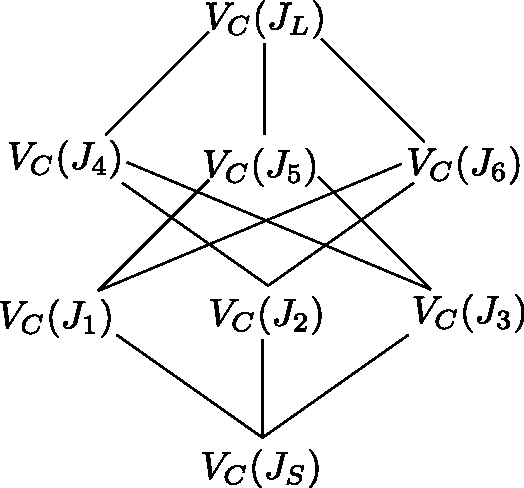
\includegraphics[width=0.8\textwidth]{interpolant_lattice.pdf}
\captionof{figure}{Interpolant lattice}
\label{Fig:int_lat}
% \begin{center}
% \end{figure}
\end{minipage}

It is easy to check  that all $V(J_I)$ satisfy the 3 conditions of
Def. \ref{def:int}. Note also that $V(J_S)$ is the smallest
interpolant, contained in every other interpolant. Likewise, $V(J_L)$
contains all other interpolants and it is the largest. The other
containment relationships are shown in the corresponding interpolant
lattice in Fig. \ref{Fig:int_lat}; i.e. $\Vc(J_1) \subset \Vc(J_5),
\Vc(J_1) \subset \Vc(J_6)$, and so on. 


 %% \begin{align*}
 %% & \Vc(J_1) \subset \Vc(J_5) ~~~~~~~~~~~~ \Vc(J_1) \subset \Vc(J_6) \\
 %% & \Vc(J_2) \subset \Vc(J_4) ~~~~~~~~~~~~ \Vc(J_2) \subset \Vc(J_6) \\
 %% & \Vc(J_3) \subset \Vc(J_4) ~~~~~~~~~~~~ \Vc(J_3) \subset \Vc(J_5)
 %% \end{align*}


}
\end{Example}



%% \begin{Example}
%% \label{example:jajb}
%% Consider the ideal $J_A$ from Example \ref{example:ja} and another
%% $J_B = \langle b,d,ec+e+c+1, ec \rangle$ with the variables of 
%% its generators partitioned as $B = \{e\}$ and $C = \{b,c,d\}$.
%% The intersection of varieties $\Vabc(J_A)$ and $\Vabc(J_B)$ is 
%% empty as,
%% \begin{align*}
%% \Vabc(J_A) &= \Fq^B \times \Vac(J_A)  \\
%% &= (abcde):\{ 01000,00010,01100,10010, \\
%% & ~~~~~~~~~~~~~~~~~~~~~~ 01001,00011,01101,10011 \} \\
%% \Vabc(J_B) &= \Fq^A \times \Vbc(J_B) \\
%% &= (abcde):\{00001,00100,10001,10100\}
%% \end{align*} 

%% Therefore, there must exist an interpolant satisfying the 
%% above three properties. 
%% \end{Example}


\begin{Theorem}
An ideal-interpolant $J_I$, and correspondingly the interpolant $\Vabc(J_I)$, as
given in Def. \ref{def:int}, always exists. 
\end{Theorem}

\begin{proof}
Consider the elimination ideal $J_I = J_A \cap \Fq[C]$. We show $J_I$ satisfies 
the three conditions for the interpolant. 

\par \noindent  \underline{Condition 1}: $\Vabc(J_I) \supseteq
\Vabc(J_A)$. This condition is trivially satisfied due  to
construction of elimination ideals. As $J_I \subseteq J_A$,
$\Vabc(J_I) \supseteq \Vabc(J_A)$.

%% In other words  any point in the $\Vabc(J_A)$ has
%% to satisfy all the polynomials in $J_I$ as $J_I$ is  a subset of
%% polynomials in $J_A$.  

\par \noindent \underline{Condition 2}: $\Vabc(J_I) \cap \Vabc(J_B) =
\emptyset$. This condition  can be equivalently stated as $\Vbc(J_I)
\cap \Vbc(J_B) = \emptyset$ as neither  $J_I$ nor $J_B$ contains any
variables from the set $A$. We prove this condition by
contradiction. Let's assume that there exists a
common point $(\mathbf{b},\mathbf{c})$ in $\Vbc(J_I)$ and $\Vbc(J_B)$.  
We know that the projection of the variety $Pr_A(\Vac(J_A))$ is equal
to the variety of the elimination ideal $\Vc(J_I)$, where $J_I=J_A
\cap \Fq[C]$, due to Lemma \ref{lemma:project}. 
 %% (as $J_A$ is radical). 
Therefore, the point $(\mathbf{c})$ in the variety of $J_I$ can be
extended to a point $(\mathbf{a},\mathbf{c})$ in the variety of
$J_A$. This implies that the ideals $J_A$ and $J_B$ vanish at 
($\mathbf{a},\mathbf{b},\mathbf{c}$). This is a contradiction to our
initial assumption that the intersection of the varieties of $J_A$ and
$J_B$ is empty.  Thus $J_I, J_B$ have no common zeros.

\par \noindent \underline{Condition 3}: The generators of $J_I$
contain only the $C$-variables. This condition is trivially satisfied
as $J_I$ is the elimination ideal obtained by  eliminating
$A$-variables in $J_A$. 
\end{proof}

The above theorem not only proves the existence of an interpolant, but
also gives a procedure to construct one: $J_I = J_A\cap\Fq[C]$. In
other words, compute a reduced Gr\"obner basis $G$ of $J_A$ w.r.t. an
elimination order $A> B > C$ and take $G_I = G \cap \Fq[C]$. Then
$G_I$ gives the generators for the ideal-interpolant $J_I$.

\begin{Example}
{\it 
The elimination ideal $J_I$ computed for $J_A$ from Example \ref{ex:main}
is $J_I = J_S = \langle cd,b+d+1 \rangle$ with variety
$\Vc(J_I)=(bcd):\{001,100,110\}$.  This variety over the variable set
$A$ and $C$ is $\Vac(J_I)=(abcd):\{0001,0100,0110, 1001,1100,1110\}$,
and it contains $\Vac(J_A)$. Moreover, $\Vabc(J_I)$ also has an empty
intersection with $\Vabc(J_B)$. 
}
\end{Example}

%The next theorem proves that this variety $\Vc(J_I)$ is also the
%smallest interpolant, $i.e.$ all other interpolants contain it. 

\begin{Theorem}
\label{thm:smallest}
The interpolant $\Vabc(J_S)$ corresponding to the ideal %-interpolant
$J_S = J_A \cap \Fq[C]$ is the smallest interpolant.
\end{Theorem}

\begin{proof} 
The proof is given in the appendix. 


%% Let $J_I \subseteq \Fq[C]$ be any another ideal-interpolant $\neq
%% J_S$. We show that $\Vc(J_S) \subseteq \Vc(J_I)$. For $\Vc(J_I)$
%% to be an interpolant it must satisfy 
%% \begin{align*}
%% \Vabc(J_A) \subseteq \Vabc(J_I)
%% \end{align*}
%% which is equivalent to 
%% \begin{align*}
%% I(\Vabc(J_A)) &\supseteq I(\Vabc(J_I)) \\
%% \implies J_A &\supseteq J_I  
%% \end{align*}
%% due to Theorem \ref{thm:strong-ns}.
%% %% as $J_I$ is radical so $I(\Vabc(J_I)) = J_I)$. 
%% As the generators of $J_I$ only contain polynomials in $C$-variables,
%% this relation also holds for the following
%% \begin{align*}
%% J_A \cap \Fq[C] &\supseteq J_I \\
%% \implies J_S &\supseteq J_I \\
%% \implies \Vc(J_S) &\subseteq \Vc(J_I).
%% \end{align*} 
\end{proof}

%After proving that the elimination ideal $J_A \cap \Fq[C]$ is the
%smallest interpolant, 
Now we discuss how the largest interpolant can be
computed. For this, we will make use of quotients of ideals. 

\begin{Definition}
\label{def:quo}
({Quotient of Ideals}) If $J_1$ and $J_2$ are ideals in a ring $R$,
then $J_1:J_2$ is the set 
%  \begin{equation}
  $\{f \in R \ |\ f\cdot g \in J_1, \forall g \in J_2\}$ %\nonumber
%  \end{equation}
and is called the {\bf ideal quotient} of $J_1$ by $J_2$.
\end{Definition}

We use ideal quotients to compute the complement of a variety. Given
an ideal $J' \subset R$ containing the vanishing polynomials, suppose
we need to find an ideal $J$ such that $V(J) = \Fq^n - V(J') = V(J_0)
- V(J')$, where ``$-$'' corresponds to the set difference
operation. Then $J = J_0 : J'$ (see Theorem III.2 and Corollary III.1
in \cite{xiaojun:hldvt2016} for a proof outline). Once again, the
Gr\"obner basis algorithm can be used to compute $J_0:J'$ 
\cite{ideals:book}.  

\begin{Theorem}
\label{thm:large}
Consider the elimination ideal $J'_L = J_B \cap \Fq[C]$. The
complement of the variety $\Vc(J'_L)$,  computed as $\Fq^C - \Vc(J'_L)$,
is the largest interpolant.
\end{Theorem}

\begin{proof} Proof is given in the appendix. 

%% We first prove that the interpolant computed by
%% complementing $\Vc(J'_L)$  as $\Fq^C - \Vc(J'_L)$ is indeed a valid
%% interpolant. As $J'_L$ is the elimination ideal computed from $J_B$,
%% $\Vbc(J'_L) \supseteq \Vbc(J_B)$. This in turn implies that the
%% complement of $V(J'_L)$ cannot intersect with $V(J_B)$ at any
%% point. This proves condition 2 for $\Fq^C - \Vc(J'_L)$ to be a
%% valid interpolant.  

%% For condition 1, we need to prove that
%% \begin{align*}
%% \Vac(J_A) \subseteq \Fq^A \times (\Fq^C - \Vc(J'_L))
%% \end{align*}
%% This can be restated as
%% \begin{align*}
%% \Vac(J_A) \cap \Fq^A \times \Vc(J'_L) = \emptyset
%% \end{align*}
%% Let us assume (by contradiction) that there exists a common point 
%% $(\mathbf{a},\mathbf{c})$ in $\Vac(J_A)$ and $\Fq^A \times
%% V_C(J'_L)$. As the projection $Pr_B(\Vbc(J_B))$ on the
%% $C$-variables is equal to  the variety of the elimination ideal
%% $\Vc(J'_L)$, a point $(\mathbf{c}) \in \Vc(J'_L)$ can be  extended to
%% some point $(\mathbf{b},\mathbf{c})$ in $\Vbc(J_B)$. This implies that
%% the point $(\mathbf{a},\mathbf{b},\mathbf{c})$ is a common point in
%% $\Vabc(J_A)$ and $\Vabc(J_B)$, which is a contradiction to our initial
%% assumption. Therefore condition 1 of Def. \ref{def:int} is satisfied
%% too and $\Fq^C - \Vc(J'_L)$ is indeed an interpolant. 

%% \par \noindent Next we prove that $\Fq^C - \Vc(J'_L)$ is the largest
%% interpolant. Consider an arbitrary ideal-interpolant $J_I$. We want to
%% prove $\Vc(J_I) \subseteq \Fq^C - \Vc(J'_L)$, or equivalently to prove
%% $\Vc(J_I) \cap \Vc(J'_L) = \emptyset$. Let us assume (by contradiction) 
%% that there exists a common point $(\mathbf{c})$ in $\Vc(J_I)$ and
%% $\Vc(J'_L)$. As $J'_L$ is the elimination ideal of $J_B$, this point
%% can be extended to some point $(\mathbf{b},\mathbf{c})$  
%% in $\Vbc(J_B)$. This in turn implies that $(\mathbf{b},\mathbf{c})$ is
%% a common point in  $\Vbc(J_B)$ and $\Fq^B \times \Vc(J_I)$. This is a
%% contradiction as an interpolant cannot intersect with the variety of
%% $J_B$. Hence, $\Fq^C - \Vc(J'_L)$ is the largest interpolant and it
%% contains all other interpolants.

\end{proof}

Let $J_L$ be the radical ideal corresponding to the largest
interpolant $\Vc(J_L) = \Fq^C - \Vc(J'_L)$. This ideal-interpolant
$J_L$ can be computed as $J_L = (J_{0,C}:J'_L)$, where $J_{0,C}$ is
ideal of vanishing polynomials in $C$-variables.  


\begin{Example}
{\it 
The ideal-interpolant $J_L = \langle bd + b + d + 1 \rangle$ in 
Example~\ref{ex:main} is computed as:
\begin{itemize}
	\item First compute the ideal $J'_L = J_B \cap \Fq[C]$ which results in 
	$J'_L = \langle b,d \rangle$.
	\item Then compute $J_L$ as $J_L = J_{0,C}: J'_L$ which results in
	$J_L = \langle bd + b + d + 1 \rangle$
\end{itemize}
The variety $V_C(J_L)=(bcd):\{001,011,100,101,110,111\}$ and it is the
largest interpolant for the given pair ($J_A,J_B$). 
}
\end{Example}

\begin{Lemma}
\label{noofinter}
The total number of interpolants for the pair ($J_A,J_B$) is
$2^{|SM(J_D)|}$, where $J_D = (J_L:J_S)$. 
\end{Lemma}

\begin{proof}
The proof is given in the appendix. 

%% The smallest and the largest interpolants are $\Vc(J_S)$ and $\Vc(J_L)$,
%% respectively. The set difference $\Vc(J_L) - \Vc(J_S)$ is also a
%% variety of some ideal $J_D$, which can be computed as
%% $J_D=(J_L:J_S)$. By selecting different subsets of $\Vc(J_D)$ and
%% adding them to $\Vc(J_S)$, we can generate all the 
%% interpolants. Consider, 
%% \begin{align*}
%% \label{eqn:pwsetjd}
%% \binom{|\Vc(J_D)|}{0} + \binom{|\Vc(J_D)|}{1} + \cdots + \binom{|\Vc(J_D)|}{|\Vc(J_D)|} = 2^{|\Vc(J_D)|}
%% \end{align*}
%% where the term $\binom{|\Vc(J_D)|}{0}$ denotes that no point is selected from $\Vc(J_D)$ and results in 
%% $\Vc(J_S)$ as the ideal-interpolant. On the other hand, the term $\binom{|\Vc(J_D)|}{|\Vc(J_D)|}$ is equivalent 
%% to selecting  all the points from $\Vc(J_D)$ and results in $J_L$ as 
%% the ideal-interpolant. So the number of interpolants is equal to
%% $2^{|\Vc(J_D)|}$. Theorem \ref{thm:count} further tells us that the 
%% cardinality of a variety of an ideal is equal to the number of
%% standard monomials of that ideal, therefore, number of interpolants $=
%% 2^{|SM(J_D)|}$.  

\end{proof}

\begin{Example}
\label{ex:jd}
{\it 
From Example~\ref{ex:main}
$J_L = \langle bd + b + d + 1 \rangle$ and $J_S = \langle cd, b + d+
1\rangle$. 
Computing $J_D = J_L : J_S$ gives $J_D = \langle
d+1,bc+b+c+1,c^2+c,b^2+b \rangle$, where the variety $\Vc(J_D)=\Vc(J_L)-\Vc(J_S)
=(bcd):\{011,101,111\}$. 

The standard monomials for $J_D$ are $SM(J_D) = \{1,b,c\}$. Therefore,
the total number of interpolants for the given pair ($J_A,J_B$) is
$2^{|\{1,b,c\}|}=2^3=8$. 
}
\end{Example}


\subsubsection{The structure of the interpolant lattice:} Note that
our results do provide some insights into the structure of the
interpolant lattice. Let $l = |SM(J_D)|$. Then, the height of the
interpolant lattice is $l + 1$, and the number of elements (interpolants) at each
level $i$ is $l \choose i$, $0\leq i \leq l$. Notice also that the size (height and
width) of the interpolant lattice is independent of the number of
variables in the set $C$, and depends only on $|SM(J_D)|$. 

%% Next we describe a procedure for enumerating all of these interpolants using the $SM(J_D)$.
%% Let's say there are $l$ standard monomials, $\{m_1,\dots,m_l\}$ in the set $SM(J_D)$. Consider
%% a polynomial $f_i$ constructed using the linear combination of $\{m_1,\dots,m_l\}$ as,
%% \begin{center}
%% $f_i = \lambda_1\cdot m_1 + \lambda_2\cdot m_2 +\cdots+ \lambda_l\cdot m_l$
%% \end{center} 
%% where each $\lambda_i \in \mathbb{F}_2$ $i.e.$ $\lambda_i \in \{0,1\}$.
%% There can be exactly $2^l$ unique polynomials obtained in this way.
%% We can then obtain all the ideal-interpolants $I_j$ as,
%% \begin{center}
%% $I_j = J_S\cdot(J_D + \langle f_i \rangle)$
%% \end{center}
%% where $\langle f_i \rangle$ is the ideal generated by the polynomial $f_i$.

\section{Enumerating the Interpolants in $\F_2[A,B,C]$}
\label{sec:alg}
Lemma~\ref{noofinter} gives us the number of interpolants that exist for the given pair 
$(J_A,J_B)$. This section presents procedures for
enumerating these interpolants using $SM(J_D)$. 
Note that these procedures can only be applied while operating over 
the field $\F_2$. First we describe a procedure for enumerating all the interpolants.
This is made possible by exploiting the relationship between 
the interpolants and $SM(J_D)$.
\begin{Theorem}
\label{thm:enum_all}
Given the interpolant setup over $\F_2[A,B,C]$, let $SM(J_D) =\{m_1,\dots,m_l\}$. 
Construct a polynomial $f_i$ 
using any linear combination of $\{m_1,\dots,m_l\}$ as, 
\begin{equation}
\label{eqn:fi}
f_i = \lambda_1\cdot m_1 + \lambda_2\cdot m_2 +\cdots+ \lambda_l\cdot m_l
\end{equation} 
where each $\lambda_j \in \mathbb{F}_2 =  \{0,1\}$.
Then all the ideal-interpolants $J_I$ can be obtained as,
\begin{equation}
\label{eqn:ji}
J_I = J_S\cdot(J_D + \langle f_i \rangle).
\end{equation}
% where $\langle f_i \rangle$ is the ideal generated by the polynomial $f_i$.
\end{Theorem}
There can be $2^l$ such $f_i$, and as $|SM(J_D)| = l$, the number of interpolants
is also $2^l$. Therefore, each $f_i$ in Eqn.~(\ref{eqn:ji}) will result in a distinct interpolant.

\begin{proof}

We want to prove that each $f_i$ will result in a 
distinct interpolant when used in Eqn.~(\ref{eqn:ji}). Consider the variety $\Vc(J_D)$
and its cardinality $|\Vc(J_D)| = l$. From the proof of Lemma~\ref{noofinter}, we know that
the union of the variety $\Vc(J_S)$ and each subset of  $\Vc(J_D)$ produces a new 
interpolant. Therefore
\begin{equation}
\label{eqn:jsuwi}
\Vc(J_I) = \Vc(J_S) \cup W_i 
\end{equation}
where $W_i \in PowerSet(\Vc(J_D))$.
\begin{figure}[hbt]
\centering
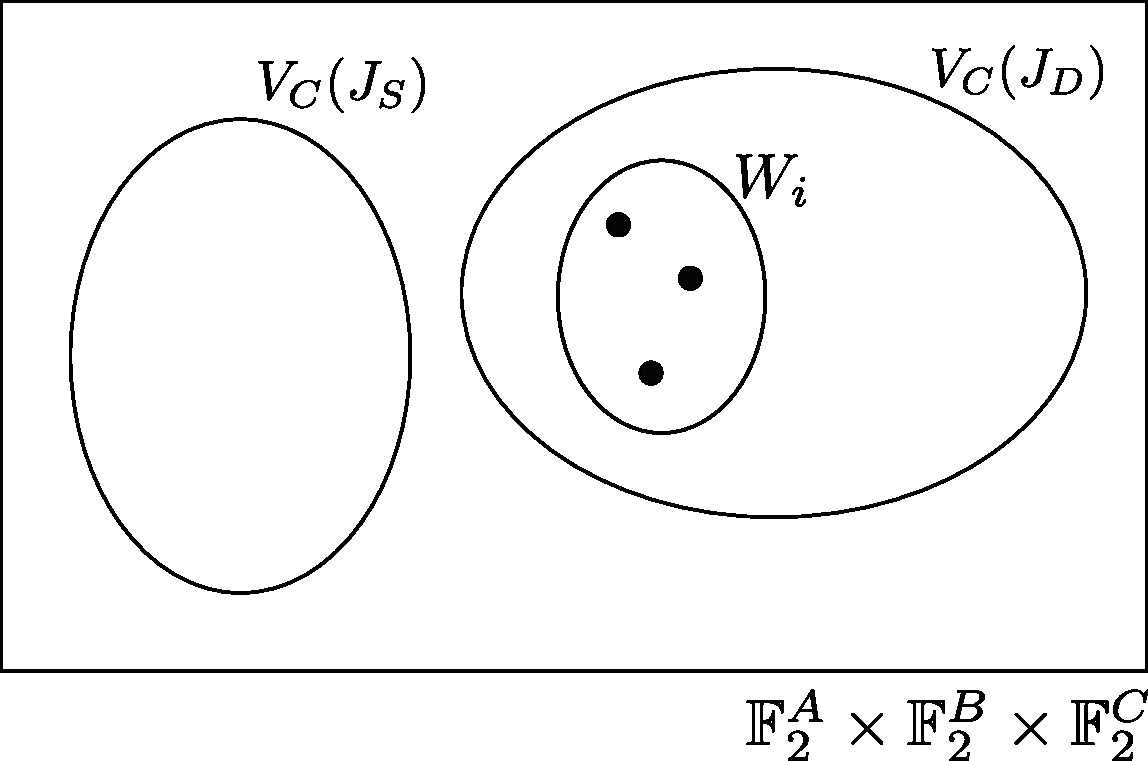
\includegraphics[scale=0.30]{vjd.pdf}
\caption{The variety $\Vc(J_D)$ and an element $W_i$ in its power set.}
\label{Fig:vjd}
\end{figure}  
\par Every $W_i$ is a set of finite number of points as shown in Fig.~\ref{Fig:vjd}, and 
therefore it forms a variety. As we are working over finite fields, the ideal of this variety 
can be constructed using only one polynomial $f'_i$. For example, $f'_i$ could be constructed by
means of Lagrange's interpolation formula over $W_i$. Therefore,
$\Vc(\langle f'_i \rangle) = W_i$. Note that there can be multiple polynomials
$f'_i$ with variety $W_i$ and they belong to the same equivalence class of polynomials
$\pmod{J_D}$. Consider the reduction $f'_i \xrightarrow{GB(J_D)} f_i$. Then
$\Vc(J_D+\langle f'_i \rangle) = \Vc(J_D + \langle f_i \rangle)$.
As $\Vc(\langle f'_i \rangle) = \Vc(J_D + \langle f'_i \rangle)$ because $\Vc
(\langle f'_i \rangle) \subseteq \Vc(J_D)$, we have $\Vc(\langle f'_i \rangle) =
\Vc(J_D + \langle f_i \rangle) = W_i$.

As $f'_i$ is reduced by 
$GB(J_D)$, the remainder $f_i \in \Fq[C]/J_D$ is a canonical representative 
for the equivalence class containing
$f'_i$ and is composed of only $SM(J_D)$. 

\par There are $2^l$ such equivalence classes of polynomials $\pmod{J_D}$ and each one of 
them can be reduced to a unique $f_i$. As there are $l$ standard monomials
$\{m_1,\dots,m_l\}$, they can be combined linearly to form $2^l$ unique polynomials $f_i$. 
Each equivalence class corresponds to a distinct interpolant (Eqn.~(\ref{eqn:jsuwi})). 
Consequently each $f_i$ will also correspond to a distinct interpolant,

\begin{align*}
\Vc(J_I) &= \Vc(J_S) \cup W_i ~~~(\text{from Eqn.~(\ref{eqn:jsuwi})}) \\
\Vc(J_I) &= \Vc(J_S) \cup (\Vc(J_d+\langle f_i \rangle)) \\
\Vc(J_I) &= \Vc(J_S) \cup (\Vc(J_d)\cap \Vc(\langle f_i \rangle)) \\
J_I &= J_S \cdot (J_D + \langle f_i \rangle) ~~~ (\text{using ideal-variety duality})
\end{align*} 

\end{proof}

\begin{Example}
\label{ex:enuall}
{\it
From Example~\ref{ex:main} and \ref{ex:jd} that are setup over $\F_2[A,B,C]$, 
we have $J_S = \langle cd, b + d+ 1 \rangle$ 
and $J_D = \langle d+1,bc+b+c+1 \rangle$ with
$SM(J_D) = \{1,b,c\}$. We can enumerate all the interpolants for the pair $(J_A,J_B)$ using
$f_i = \lambda_1\cdot 1 + \lambda_2\cdot b + \lambda_3\cdot c$ 
where $\{\lambda_1,\lambda_2,\lambda_3\} \in \{0,1\}$. 
\begin{itemize}
	\item Let $f_1 = c$ with $(\lambda_1,\lambda_2,\lambda_3)=(0,0,1)$.\\
	The GB computation 
	of the ideal $J_S\cdot (J_D + \langle f_1 \rangle)$ results in 
	$\langle cd,bd+b+d+1,bc+cd+c \rangle$ ~~ (= $J_1$ from Example~\ref{ex:main}) 
	\item Let $f_5 = b+1$ with $(\lambda_1,\lambda_2,\lambda_3)=(1,1,0)$. \\
	The GB computation 
	of the ideal $J_S\cdot (J_D + \langle f_5 \rangle)$ results in 
	$\langle bc+c,bd+b+d+1 \rangle$ ~~ (= $J_5$ from Example~\ref{ex:main})
	\item Let $f_6 = b+c+1$ with $(\lambda_1,\lambda_2,\lambda_3)=(1,1,1)$. \\
	The GB computation 
	of the ideal $J_S\cdot (J_D + \langle f_6 \rangle)$ results in 
	$\langle bd+b+d+1,bc+cd+c \rangle$ ~~ (= $J_6$ from Example~\ref{ex:main})
	\item Similarly, all the 8 interpolants can be obtained from the
	8 possible $f_i$.
\end{itemize}
}
\end{Example}

The reason why Theorem~\ref{thm:enum_all} requires the interpolant setup over $\F_2[A,B,C]$ is as follows.
If we assume that the setup was over some other finite field $\Fq$, then Eqn.~(\ref{eqn:fi}) will 
produce $q^l$ $(l=|SM(J_D|)$ polynomials $f_i$. However, the number of interpolants is exactly equal 
to $2^l$ irrespective of the field we are working on (Lemma~\ref{noofinter}). As a result, multiple 
$f_i$ can produce same interpolant unlike the case when $q=2$ (each $f_i$ produces a distinct interpolant).
The study to enumerate all the interpolants for any finite field using the $SM(J_D)$ 
is a part of our future work.


\par In practice, we don't need to compute all interpolants. However, given an interpolant it may
be desirable to obtain a larger interpolant that provides a better abstraction.
Given an ideal-interpolant $J_I$ we discuss how a larger 
ideal-interpolant $J_K$ can be obtained so that $\Vc(J_I) \subset \Vc(J_K)$.

\par Let $J_I$ and $J_K$ be two ideal-interpolants obtained using polynomials
$f_i$ and $f_k$ respectively (using Eqn. (\ref{eqn:ji})). Assuming that 
$\Vc(J_I) \subset \Vc(J_K)$ consider,
\begin{align*}
\Vc(J_I) &\subset \Vc(J_K) \\
\Vc(J_S\cdot(J_D + \langle f_i \rangle)) &\subset \Vc(J_S\cdot(J_D + \langle f_k \rangle)) \\ 
\Vc(J_S) \cup \Vc(J_D + \langle f_i \rangle) &\subset \Vc(J_S) \cup \Vc(J_D + \langle f_k \rangle)
\end{align*}
\par \noindent as the sets $\Vc(J_S)$ and $\Vc(J_D)$ are disjoint (Fig.~\ref{Fig:vjd}) we can
write
\begin{align*}
\label{eqn:chainofinter}
\Vc(J_D + \langle f_i \rangle) &\subset \Vc(J_D + \langle f_k \rangle) \\
I(\Vc(J_D + \langle f_i \rangle)) &\supset I(\Vc(J_D + \langle f_k \rangle)) 
\end{align*}
using Lemma~\ref{lemma:radical-ff} and Theorem~\ref{thm:strong-ns} we have
\begin{align}
\begin{split}
J_D + \langle f_i \rangle &\supset J_D + \langle f_k \rangle \\
J_D + \langle f_i \rangle &\supset f_k
\end{split}
\end{align}  
% If the interpolant $\Vc(J_i)$ is contained in some other interpolant 
% computed using  $f_j$, then the relation in Eqn.~\ref{eqn:chainofinter} 
% is also true for that $f_j$. 
\par Now that we know that $f_k$ is contained in $J_D + \langle f_i \rangle$,
we will show how $f_k$ can be obtained from the GB of $J_D + \langle f_i \rangle$.

\begin{Theorem}
\label{thm:chainofinter}
Given an ideal-interpolant $J_I$ computed as $J_I = J_S\cdot(J_D + \langle f_i \rangle)$. Obtain the
reduced $GB$ $G_{Di}=GB(J_D + \langle f_i \rangle)$. Then there must exist 
at least one $g_j \in
G_{Di}$ which is a linear combination of $SM(J_D)$. 
Each $g_j \neq f_i$ can be used to 
obtain a new interpolant $J_K$ such that
$\Vc(J_I) \subset \Vc(J_K)$.  
\end{Theorem}

\begin{proof} 
We need to show that $G_{Di}$ will contain 
at least one polynomial that is a  linear combination of $SM(J_D)$.
As a reduced $GB$ is a canonical representation, $G_{Di}$ 
can also be computed as $GB(GB(J_D) + \langle f_i \rangle)$. 
Consider the set $GB(J_D)$
where each polynomial $p_r$ can be written as $lt(p_r) + (p_r - lt(p_r))$. 
The monomials in $p_r-lt(p_r)$ can only contain the elements of $SM(J_D)$ 
(otherwise they can be divided by the leading terms of polynomials in $J_D$).

\par Construct $GB(J_D) + \langle f_i \rangle$ and compute the 
reduced $GB$ of this ideal. As the set of polynomials $GB(J_D)$ is already a 
$GB$, Buchberger's algorithm will pair $f_i$ and each polynomial from the set
$GB(J_D)$ for the $S$-$poly$ computation $S$-$poly(p_r,f_i) \xrightarrow{GB(J_D),f_i}_+ h_r$. 
The $S$-$poly$ is reduced modulo $\{GB(J_D), f_i\}$ 
and as a result $h_r$ will only be composed of $SM(J_D)$. 
% If the reduced S-poly 
% contains some monomials $\not \in SM(J_D)$, then they will be reduced by some 
% polynomial in $GB(J_D)$. 
This implies that there will be at least one polynomial
in the $GB(J_D + \langle f_i \rangle))$ containing monomials only from the set $SM(J_D)$. 
This polynomial can then be used to compute an ideal-interpolant $J_K$ such that 
$\Vc(J_I) \subset \Vc(J_K)$.

% Let's say we perform the S-poly computation for some $p_r$ and $f_i$. This will result
% in an expression like $\beta \cdot tail(p_r) + \alpha \cdot tail(f_i)$ where 
% $\alpha = LCM(lt(f_i),lt(p_r))/lt(f_i)$ and $\beta  = LCM(lt(f_i),lt(p_r))/lt(p_r)$. This S-poly 
% is then reduced modulo each polynomial $p_r$ and $f_i$. The monomials of this remainder can
% only be elements from $SM(J_D)$ and can be used to obtain a larger interpolant (Eqn.~\ref{eqn:ji}).  
% Also there always be at least one such polynomial otherwise it would imply $f_i \in J_D$ ($i.e.$ all the S-poly are zero).
% This is not possible as $f_i$ is constructed using the $SM(J_D)$. If there is only one polynomial
% in $G_{Di}$ which is a linear combination of $SM(J_D)$ and is $f_i$ itself, then using 
% this polynomial in Eqn.~\ref{eqn:ji} will result in $f_i$ itself. In that case, the only larger interpolant
% is $J_L$ itself.   
% \end{proof}

\end{proof}

If there is only one polynomial
in $G_{Di}$ which is a linear combination of $SM(J_D)$ and is $f_i$ itself, then using 
this polynomial in Eqn.~(\ref{eqn:ji}) will result in $J_I$ itself. In that case, 
the only larger interpolant is $J_L$.

\par Theorem \ref{thm:chainofinter} gives an approach to devise an algorithm that computes a chain of progressively larger interpolants starting from $J_S$. The following steps explain the algorithm.
\begin{enumerate}
	\item Given the pair $(J_A,J_B)$ in $\F_2[A,B,C]$, compute $J_S$, $J_D$, 
	and $SM(J_D)$. Store $J_S$ in some list $L$.
	\item Pick a polynomial $f_i = \sum_{i=1}^{i=l} \lambda_i \cdot m_i$, 
	where $\{m_1, \dots,m_l\} = SM(J_D)$ and $\lambda_i \in \{0,1\}$. ($f_i \neq 1$ otherwise,
	$GB(J_D + \langle 1 \rangle) =1$, so $J_I = J_S$).
	\item Compute $G_{Di} = GB(J_D + \langle f_i \rangle)$. Append $J_I = J_S\cdot G_{Di}$
	to $L$.
	\item In $G_{Di}$ find polynomials $g_j$ which are of the 
	form $\sum_{i=1}^{i=l} \lambda_i \cdot m_i$.
	\item Pick a $g_j \neq f_i$ and goto step 3 where $g_j$ replaces $f_i$
	in the computation of $G_{Di}$.
	\item If in step 4, there is only one $g_j$ and $g_j = f_i$,
	terminate the algorithm after appending $J_L = J_S \cdot J_D$ to $L$.
\end{enumerate} 
The algorithm returns the list $L$ whose first element is $J_S$ and last element is
$J_L$ with a chain of progressively larger interpolants in between.
The pseudo-code for this algorithm is presented in Algorithm~\ref{algo:chainofinter}. 


% The inputs are the ideals $J_S$, $J_D$, and the polynomial $f_i$. 
% The algorithm initializes a list $L$ that will store the interpolants computed by the algorithm. The infinite while 
% loop terminates when there is only one $g_j$ in $G_{Di}$ and $g_j = f_i$. In that case, the algorithm appends
% $J_L = J_S\cdot J_D$ to $L$ and returns $L$. Otherwise, it picks one $g_j$, appends the corresponding ideal-interpolant 
% to $L$ and re-iterates with $G_{Di} = GB((J_D + \langle g_j \rangle))$.

\begin{algorithm}
\caption{Compute larger ideal-interpolants given $J_I \neq J_S$}
\label{algo:chainofinter}
\begin{algorithmic}[1]

\Procedure{$get\_larger\_interpolant$}{$J_S,J_D,SM(J_D)$}
\State {\it Initialize list $L$ for storing interpolants}
\State {\it Append $J_S$ to $L$}
\State {\it Pick $f_i = \sum_{i=1}^{i=l} \lambda_i \cdot m_i ~~~ (f_i\neq 1)$}
\While{(1)}
\State Compute $G_{Di} = GB(J_D + \langle f_i \rangle)$ 
\State {\it Append $J_S\cdot G_{Di}$ to $L$}
\State {\it Find $g_j \in G_{Di}$ $s.t.$ $g_j = \sum_{i=1}^{i=l} \lambda_i \cdot m_i$}
\If{\it $|\{g_j\}| = 1$ and $g_j = f_i$}
\State {\it Append $J_S\cdot J_D$ to $L$}
\State \Return $L~~$ {\it //Reached largest interpolant}
\Else
\State {\it Choose a $g_j \neq f_i$}
\State {\it $f_i = g_j$}
% \State $G_{Di} = GB(J_D + \langle g_j \rangle)$
\EndIf

\EndWhile
% \State \Return $L$
\EndProcedure

\end{algorithmic}
\end{algorithm}

\begin{Example}
\label{ex:chainofinter}
{\it
The algorithm can be understood with this example. Consider the following steps.
\begin{itemize}
	\item From Example \ref{ex:jd}, $J_S = \langle cd, b + d+ 1 \rangle$,
	$J_D = \langle d+1,bc+b+c+1 \rangle$ with $SM(J_D) = \{1,b,c\}$. The ideal-interpolant $J_S$
	is appended to $L$ so that $L = [J_S]$.
	
	\item We need to pick a $f_i = \lambda_1\cdot 1 + \lambda_2\cdot b + \lambda_3\cdot c$ and
	$f_i \neq 1$. Let $f_1 = c$ with $(\lambda_1,\lambda_2,\lambda_3) = (0,0,1)$.
	
	\item The computation $G_{Di} = GB(J_D + \langle f_1 \rangle)$ results in the ideal
	$G_{Di} = \langle d+1,b+1,c \rangle$. The ideal-interpolant $J_1 = J_S \cdot G_{Di}$ 
	(same as the $J_1$ in Example~\ref{ex:enuall}) is appended to 
	$L$ so that $L = [J_S,J_1]$.
	
	\item In $G_{Di}$, the only $g_j$ of the form $\sum_{i=1}^{i=l} \lambda_i \cdot m_i$ are
	$g_1 = b+1$ and $g_2 = c$. 

	\item We select $g_1$ for the computation of larger interpolant as $g_2 = f_1$. Notice that $g_1$ is equal to $f_5$ from Example ~\ref{ex:enuall}.
	
	\item Using $g_1$ in the computation $GB(J_D + \langle g_1 \rangle)$ results in the
	ideal $\langle d+1, b+1\rangle$. Also the ideal-interpolant $J_5 = J_S\cdot (J_D + \langle g_1 
	\rangle) = J_S\cdot (J_D + \langle f_5) \rangle$ is appended to $L$ so that $L = [J_S,J_1,J_5]$.
	
	\item The only $g_i$ in $GB(J_D + \langle g_1 \rangle) = \langle d+1, b+1\rangle$ of the 
	form $\sum_{i=1}^{i=l} \lambda_i \cdot m_i$ is $b+1$. As $b+1 = f_5$, the only larger
	interpolant for $J_5$ is $J_L$. Therefore, the algorithm returns the $L = [J_S,J_1,J_5,J_L]$.

\end{itemize}
% From Example~\ref{ex:main}, we have $\Vc(J_1) \subset \Vc(J_5)$ and $\Vc(J_1) \subset \Vc(J_6)$. From 
% Example~\ref{ex:enuall}, we also know that $f_1 = c,~f_5 = b+1,$ and $f_6 = b + c + 1$ and the ideal $J_D$. 
% The computation $GB(J_D + \langle f_1 \rangle)$ results in the ideal $\langle d+1,b+1,c \rangle$. We have
% $g_1 = b+1$ and $g_2 = c$ as linear combinations of $SM(J_D)$. Notice that $g_1 = f_5$ and performing
% the computation $J_S\cdot(J_D + \langle g_1 \rangle)$ will result in $J_5$. Also $g_2 = f_1$, so we will
% not consider it in the computation of a larger interpolant. However, the linear combination $g_1 + g_2 = f_6$
% is also a suitable candidate for obtaining a larger interpolant and results in $J_6$.
% \par The computation $J_D + \langle f_5 \rangle$ results in $\langle d+1, b+1\rangle$. We only have one $g_1$
% as linear combinations of $SM(J_D)$ and $g_1 = f_5$. Therefore, the only larger interpolant for $\Vc(J_5)$ is
% $J_L$. Same is also true for $J_6$.

}

\vspace{0.1in}
\end{Example}

%% \par \noindent \underline{Discussions:} 
%% \begin{itemize}
%% \item The theorems and algorithm presented 
%% in the sections \ref{sec:theory} and \ref{sec:alg} make use of Gr\"obner basis concepts
%% and rely on GB computation. The computational complexity of
%% Buchberger's algorithm is exponential making these theorems practically infeasible. 
%% \par GB concepts are being extensively used in the verification of hardware circuits. 
%% When operating over Boolean circuits, \cite{pruss:tcad} and \cite{xiaojun:hldvt2016}
%% describe a topological monomial order that can be 
%% derived from the gates of the circuit. This order obviates the need to explicitly compute a 
%% Gr\"obner basis and the overall complexity is dictated by polynomial reductions. 
%% \par We are currently working on orderings and heuristics that can avoid GB computation complexity
%% when the Craig interpolants are used for circuit based applications like logic synthesis.
%% However, before these techniques can be applied to circuits, a theory of
%% Craig interpolants in finite fields needs to be set in place which 
%% is the primary purpose of this paper.

%% \item As an improvement to our approach, the step in line 13 of Algorithm~\ref{algo:chainofinter} can use improved heuristic 
%% when choosing a $g_j$. Instead of selecting just one $g_j$ of the form $\sum_{i=1}^{i=l} \lambda_i \cdot m_i$,
%% one can also select a linear combination of multiple $g_j$ as long as this combination does not
%% compute to $f_i$. This is because the combination of multiple $g_j$ is still of the
%% form $\sum_{i=1}^{i=l} \lambda_i \cdot m_i$. 
%% \par From Example \ref{ex:main} we know that $\Vc(J_1) \subset \Vc(J_5)$
%% and $\Vc(J_1) \subset \Vc(J_6)$. We also saw in the Example \ref{ex:chainofinter} that we can
%% obtain $J_5$ by selecting $g_1 = b+1$ from the set $GB(J_D + \langle f_1 \rangle)$. If we consider the linear 
%% combination $g_3$ of $g_1$ and $g_2$ obtained as $g_3 = g_1 + g_2 = b+c+1$, then from Example \ref{ex:enuall},
%% $g_3 = f_6$ and can be used to compute $J_6$. 

%% \end{itemize} 

% \begin{Theorem}
% Given an ideal-interpolant $I_j$ computed using the Theorem~\ref{enum_all} and the polynomial
% $f_j$ (linear combination of $SM(J_D)$,
% \begin{enumerate}
% 	\item Compute reduced $GB$ of $(J_D + \langle f_j \rangle)$
% 	\item The $GB(J_D + \langle f_j \rangle)$ will contain some 
% 	polynomials $h_1,\dots,h_r$ that are linear combinations of
% 	$SM(J_D)$. 
% 	\item Use Theorem~\ref{enum_all} and each of these $h_i$
% 	or their linear combinations to obtain interpolants that contain 
% 	$\Vc(I_j)$.
% \end{enumerate}
% \end{Theorem}
% After obtaining a larger ideal-interpolant $I_k$ we can using this
% theorem again to obtain an interpolant which is larger than $\Vc(I_k)$.
% We may encounter a $h_i$ exactly equal to $f_j$ (the polynomial 
% used for computing $I_j$). We will avoid using this $h_i$ as it will
% result in $I_j$ itself.  

\section{Experiments}
\label{sec:exp}

This section presents experimental results using our approach to debug
the circuits and perform a single-fix rectification. 
We compare results of our implementation against the incremental SAT-based approach presented in~\cite{fujita:2015} wherever it's relevant.
The approach presented in~\cite{fujita:2015} is implemented using PICOSAT~\cite{picosat}. The experiments were performed on a 3.5GHz 
Intel(R) $\text{Core}^{\text{TM}}$ i7-4770K Quad-Core CPU with 32 GB of RAM. The data-path sizes {$k$} are selected according to cryptography standards recommended by U.S. National Institute of Standards and Technology (NIST). 
% In our experiments, the labels $NO$, $NM$, and $NI$ denote 
% % the location of unknown component within the circuit topology. Here $NI$, $NM$, and $NO$ 
% that the unknown component is near the input, middle, and near the output, respectively.
We have performed experiments for the cases when the bugs  are present near 
the input, middle, or near the output of the circuit, represented
using labels $NI$, $NM$, and $NO$ respectively in the tables. All the algorithms
were implemented in SINGULAR~\cite{DGPS}. 

%\subsection{Word level specification v/s Gate level implementation}

\subsubsection{Verification between a word level specification v/s Mastrovito implementation}
~\autoref{masvsspec} presents the results of our approach when the bugs are placed
in a Mastrovito multiplier implementation compared against a specification, which is given in terms of a word level polynomial $f$. 
A Mastrovito multiplier has word level specification $Z = A\times B \pmod{ P(x)}$, 
where $P(x)$ is a given primitive polynomial for the datapath size $k$. The product $A \times B$ 
is computed using an array multiplier architecture, and then the result is reduced modulo $P(x)$. 
Bugs in the circuit are introduced, and the presence of the bugs is
detetced. Then we apply our approach to check for single-fix
rectification interatively on the nets selected in $\mathcal{N}$. If
rectification is feasible at $x_i$, the unknown component problem is
solved to identify a rectification function. 

%% The circuit implementation is modeled as a set of polynomials $F=\{f_1,\dots f_i,\dots,f_s\}$. The 
%% approach then follows the partial reduction of specification polynomial $f$ until leading term of $f_i$ while
%% recording the intermediate quotients and remainders. We then represent the partial remainder as a linear combination
%% using the remaining gate polynomials and the quotient to obtain the solution $P$.
We 
are able to verify and debug the circuits for upto 64-bits within our
stipulated Time Out ($TO$)  period.

\begin{table*}[hbt]
\centering
\caption{{\small Single fix rectification debug in Mastrovito circuit against word level specification}. Time is in seconds; $k$ = Datapath Size, \#Gates = No. of gates, K = $10^3$, \textit{a}=verification time, \textit{b}=time for rectification check, \textit{c}=time for component correction computation,\textit{d}=total time}
\label{masvsspec}
\begin{tabular}{| c | c | c | c | c | c | c | c | c | c | c | c | c | c |} \hline
\multirow{3}{*}{\textbf{k}}& \multirow{3}{*}{\#Gates} & \multicolumn{12}{ c |}{Our implementation}\\ \cline{3-14}
&&\multicolumn{4}{ c |}{\it NI}&\multicolumn{4}{ c |}{\it NM}&\multicolumn{4}{ c |}{\it NO}\\ \hline
&&{\it a}&{\it b}&{\it c} &{\it d}&{\it a}&{\it b}&{\it c} &{\it d}&{\it a}&{\it b}&{\it c} &{\it d}\\ \hline
9 & 0.23K & 0.0 & 0.0 & 0.0 & 0.0 & 0.0 & 0.0 & 0.0 & 0.0 & 0.0 & 0.0 & 0.0  & 0.0\\ \hline
10& 0.29K & 0.0 & 0.0 & 0.0 & 0.0 & 0.0 & 0.0 & 0.0 & 0.0 & 0.0 & 0.0 & 0.0  & 0.0\\ \hline
11& 0.35K & 0.0 & 0.0 & 0.1 & 0.1 & 0.0 & 0.0 & 0.1 & 0.1 & 0.0 & 0.0 & 0.1  & 0.1\\ \hline
12& 0.97K & 0.1 & 0.5 & 0.4 & 0.9 & 0.2 & 0.5 & 0.4 & 1.1 & 0.5 & 0.8 & 0.4  & 1.7\\ \hline
13& 0.82K & 0.1 & 0.3 & 0.2 & 0.6 & 0.2 & 0.6 & 0.2 & 1.0 & 0.7 & 0.8 & 0.2  & 1.7\\ \hline
16& 1.8K  & 0.9 & 2.6 & 1.0 & 4.5 & 1.1 & 3.5 & 1.0 & 5.6 & 2.8 & 5.3 & 1.0  & 9.1\\ \hline
32& 5.4K  & 36  & 110 & 42  & 188 & 40  & 160 & 47  & 247 & 38  & 240 & 150  & 428\\ \hline
64& 21.8K & 2210& 7100 & 2432 & 9532 & 2200 & 8000 & 2575 & 12775 & 2150& 7840 & 10020 & 20010 \\ \hline
\end{tabular}
\end{table*}


\begin{table*}[hbt]
\centering
\caption{{\small Rectification for Mastrovito circuit with Montgomery circuit as specification}. Time is in seconds; $k$ = Datapath Size, \#Gates = No. of gates, (TO): Time-Out = 3 hrs, K = $10^3$,\textit{a}=verification time, \textit{b}=time for rectification check, \textit{c}=time for component correction computation, \textit{d}=total time}
\label{masusmontspec}
\begin{tabular}{| c | c |  c | c | c | c | c | c | c | c | c | c | c | c | c | c | c |} \hline
\multirow{4}{*}{\textbf{k}}& \multirow{4}{*}{\#Gates} & \multicolumn{3}{ c |}{Incremental SAT\textbf{~\cite{fujita:2015}}}& \multicolumn{12}{ c |}{Our Approach}\\ \cline{3-17}
&&\multirow{2}{*}{\it NI}&\multirow{2}{*}{\it NM}&\multirow{2}{*}{\it NO}&\multicolumn{4}{ c |}{\it NI}&\multicolumn{4}{ c |}{\it NM}&\multicolumn{4}{ c |}{\it NO} \\ \cline{6-17}
&&&&&{\it a}&{\it b}&{\it c} &{\it d}&{\it a}&{\it b}&{\it c} &{\it d}&{\it a}&{\it b}&{\it c} &{\it d}\\ \hline
9 & 0.6K & 35   & 37   & 33    & 0.1 & 0.5 & 0.2 & 0.8 & 0.2 & 0.2 & 0.1 & 0.5 & 1.8 & 2.2 & 0.6 & 4.6 \\ \hline
10& 0.7K & 231  & 215  & 214   & 0.3 & 1   & 0.5 & 1.8 & 0.3 & 1   & 0.8 & 2.1 & 4.7 & 5.4 & 0.2 & 10 \\ \hline
11& 0.9K & 2090 & 1927 & 2000  & 0.6 & 2   & 1   & 3.6 & 0.8 & 2   & 32  & 35  & 9 & 10 & 0.4 & 19 \\ \hline
12& 1.6K & 8676 & 23400& 24085 & 3.2 & 9.6 & 3.5 & 16  & 3.2 & 9.3 & 12  & 24  & 155 & 160 & 1.6 & 316 \\ \hline
13& 1.7K & TO   & TO   & TO    & 3.3 & 10  & 4.5 & 18  & 3.5 & 10 & 22 & 35 & 170 & 177 & 1.6 & 349 \\ \hline
16& 3K   & TO   & TO   & TO    & 27  & 81  & 35  & 143 & 28 & 83 & 48 & 159 & 210 & 176 & 2.5 & 389\\ \hline
32& 9.8K & TO   & TO   & TO    &  2060   & 6595    & 1870&  10525   & 2100 & 7320 & 1289 & 10709 & 2215 & 7870 & 1204 & 11289 \\ \hline
\end{tabular}
\end{table*}




% \begin{table}[H]
% \centering
% \caption{{Single fix rectification debug in Mastrovito circuit against word level specification}. Time is in seconds; $k$ = Datapath Size, \#Gates = No. of gates, K = $10^3$}
% \label{masvsspec}
% \begin{tabular}{| c | c | c | c | c | c | c | c | c | c | c | c | c | c | c | c | c |} \hline
% \multirow{3}{*}{\textbf{k}}& \#Gates & \multicolumn{15}{ c |}{Our implementation}\\ \cline{3-17}
% &&\multicolumn{5}{ c |}{\it NI}&\multicolumn{5}{ c |}{\it NM}&\multicolumn{5}{ c |}{\it NO}\\ \hline
% &&{\it a}&{\it b}&{\it c} &{\it d}&{\it e}&{\it a}&{\it b}&{\it c} &{\it d}&{\it e}&{\it a}&{\it b}&{\it c} &{\it d}&{\it e}\\ \hline
% 9& 0.23K & 0.0 & 0.1 & 0.0 & 0.2 & 0.0 & 0.1 & 0.0 & 0.2 & 0.0 & 0.2 & 0.0 & 0.3\\ \hline
% 10& 0.29K & 0.0 & 0.3 & 0.0 & 0.3 & 0.0 & 0.3 & 0.0 & 0.3 & 0.0 & 0.4 & 0.0 & 1.4\\ \hline
% 11& 0.35K & 0.0 & 0.2 & 0.0 & 0.3 & 0.0 & 0.3 & 0.0 & 0.4 & 0.0 & 0.6 & 0.0 & 0.7\\ \hline
% 12& 0.97K & 0.1 & 7.5 & 0.5 & 8.0 & 0.2 & 10.1 & 0.5 & 10.5 & 0.5 & 121.2 & 0.8 & 121.3\\ \hline
% 13& 0.82K & 0.1 & 4.3 & 0.3 & 4.5 & 0.2 & 11.3 & 0.6 & 11.2 & 0.7 & 156.3 & 0.8 & 158.1\\ \hline
% 16& 1.8K & 0.9 & 14.1 & 2.6 & 30.2 & 1.1 & 33.1 & 3.5 & 34.9 & 2.8 & 501.2 & 5.3 & 503.0\\ \hline
% 32& 5.4K & 36.8 & 378.6 & 110.5 & 544.7 & 40.0 & 567.1 & 160.3 & 767.2 & 38.1 & 1286.1 & 240.3 & 1342.7\\ \hline
% %64& 21.8K & 36.8 & 378.6 & 110.5 & 544.7 & 40.0 & 567.1 & 160.3 & 767.2 & 38.1 & 1286.1 & 240.3 & 1342.7\\ \hline
% \end{tabular}
% \end{table}

\subsubsection{Word level specification v/s Point addition implementation}
Point addition is an important operation required for the task of encryption, decryption 
and authentication in Elliptic Curve Cryptography (ECC). 
Modern approaches represent the points in projective
coordinate systems, {\it e.g.}, the L$\acute{o}$pez-Dahab (LD) projective coordinate, due to which the point addition 
operation can be implemented as polynomials in the field.

\begin{Example}
{\it\small %Consider point addition in L$\acute{o}$pez-Dahab (LD) projective
  %coordinate.
  Given an elliptic curve: $Y^2 + XYZ = X^3Z + aX^2Z^2 +
  bZ^4$ over $\mathbb{F}_{2^k}$, where $X,Y,Z \in \mathbb{F}_{2^k}$ and similarly, $a, b$ are
  constants from the field. Point addition over the
  elliptic curve is ($X_3$, $Y_3$, $Z_3$) = ($X_1$, $Y_1$, $Z_1$) +
  ($X_2$, $Y_2$, $1$).  Then $X_3$, $Y_3$, $Z_3$ can be computed as
  follows:}
\vspace{-0.09in}
{\tiny
\begin{align*}
&A = Y_2 \cdot Z_1^2 + Y_1  &&B = X_2 \cdot Z_1 + X_1 \\
&C = Z_1 \cdot B  &&D = B^2 \cdot(C + a Z_1^2) \\
&Z_3 = C^2 && E = A \cdot C  \\
&X_3 = A^2 + D + E &&F = X_3 + X_2 \cdot Z_3 \\
&G = X_3 + Y_2\cdot Z_3 && Y_3 = E\cdot F + Z_3 \cdot G
\end{align*}
}
\vspace{-0.38in}

\end{Example}

Each of the polynomials in the above design are implemented as a
(gate-level) logic block and are interconnected to obtain final
outputs $X_3,Y_3$ and $Z_3$. ~\autoref{pdvsspec} shows
the comparison of the time required for debugging and rectification
for the implementation of the block $D= B^2\cdot(C + aZ_1^2)$. 

\begin{table}[H]
\centering
\caption{{\small Single fix rectification debug in Point Addition circuits against word level specification}. Time is in seconds; $k$ = Datapath Size, \#Gates = No. of gates, K = $10^3$, \textit{a}=verification time, \textit{b}=time for rectification check,\textit{c}=time for component correction computation,\textit{d}=total time}
\label{pdvsspec}
\begin{tabular}{| c | c | c | c | c | c | c | c | c | c | c | c | c | c |} \hline
\multirow{3}{*}{\textbf{k}}& \multirow{3}{*}{\#Gates} & \multicolumn{12}{ c |}{Our implementation}\\ \cline{3-14}
&&\multicolumn{4}{ c |}{\it NI}&\multicolumn{4}{ c |}{\it NM}&\multicolumn{4}{ c |}{\it NO}\\ \hline
&&{\it a}&{\it b}&{\it c} &{\it d}&{\it a}&{\it b}&{\it c} &{\it d}&{\it a}&{\it b}&{\it c} &{\it d}\\ \hline
8 & 244  & 0.0 & 0.0 & 0.0 & 0.0 & 0.0 & 0.0 & 0.0 & 0.0 & 0.0 & 0.0 & 0.0 & 0.0\\ \hline
16& 1.2K & 1.3 & 3.9 & 1.5 & 6.7 & 1.2 & 3.7 & 2   & 6.9 & 1.2 & 3.7 & 1.8 & 6.7\\ \hline
32& 3.9K & 37  & 112 & 77  & 226 & 38  & 110 & 22  & 170 & 37  & 108 & 35  & 180\\ \hline
%64& 15K  & 40  & 2283&  &  &  &  &  &  &  &  &   & \\ \hline
\end{tabular}
\end{table}

\subsubsection{Word level specification v/s Barrett reduction implementation}
Barrett reduction
%~\cite{barrett}
is the other widely used multiplier design
method adopted in cryptography system designs. 
Based on Barrett reduction, a multiplier can be designed in two steps:
multiplication $R = A \times B$ and a subsequent Barrett reduction G =
R (mod P). ~\autoref{bartvsspec} shows results for debugging and rectification of
Barrett multipliers against a polynomial specification. 

\begin{table}[H]
\centering
\caption{{\small Single fix rectification debug in Barrett reduction circuits against word level specification}. Time is in seconds; $k$ = Datapath Size, \#Gates = No. of gates, K = $10^3$, \textit{a}=verification time, \textit{b}=time for rectification check,\textit{c}=time for component correction computation,\textit{d}=total time}
\label{bartvsspec}
\begin{tabular}{| c | c | c | c | c | c | c | c | c | c | c | c | c | c |} \hline
\multirow{3}{*}{\textbf{k}}& \multirow{3}{*}{\#Gates} & \multicolumn{12}{ c |}{Our implementation}\\ \cline{3-14}
&&\multicolumn{4}{ c |}{\it NI}&\multicolumn{4}{ c |}{\it NM}&\multicolumn{4}{ c |}{\it NO}\\ \hline
&&{\it a}&{\it b}&{\it c} &{\it d}&{\it a}&{\it b}&{\it c} &{\it d}&{\it a}&{\it b}&{\it c} &{\it d}\\ \hline
8 & 134 & 0.0 & 0.0 & 0.0 & 0.0 & 0.0 & 0.0 & 0.0 & 0.0 & 0.0 & 0.0 & 0.0 & 0.0\\ \hline
16& 427 & 0.1 & 0.0 & 0.0 & 0.1 & 0.0 & 0.2 & 0.1 & 0.3 & 0.0 & 0.1 & 0.3 & 0.4\\ \hline
32& 1.4K & 0.4 & 1.4 & 0.1 & 1.9 & 0.5 & 1.5 & 0.1 & 2.1 & 1.2 & 2.2 & 1.1 & 4.5\\ \hline
64& 4.9K & 19  & 58  & 5.4 & 82  & 21  & 60  & 1.7 & 83  & 63  & 104 & 141 & 308\\ \hline
\end{tabular}
\end{table}

Since the SAT-based approach cannot be applied against a word level specification polynomial, 
we perform experiments while using another multiplier implementation as the specification.

\subsubsection{Verification between a specification and implementation
  given as gate level circuits: Mastrovito v/s Montgomery multipliers}

%% \begin{table*}[ht]
%% \centering
%% \caption{{Resolving Unknown Component in Mastrovito circuit with Montgomery circuit as specification}. Time is in seconds; $k$ = Datapath Size, \#Gates = No. of gates, (TO): Time-Out = 3 hrs, K = $10^3$,\textit{a}=verification time, \textit{b}=time for rectification check,\textit{c}=time for component correction computation,\textit{d}=total time}
%% \label{masusmontspec}
%% \begin{tabular}{| c | c |  c | c | c | c | c | c | c | c | c | c | c | c | c | c | c |} \hline
%% \multirow{4}{*}{\textbf{k}}& \multirow{4}{*}{\#Gates} & \multicolumn{3}{ c |}{Incremental SAT\textbf{~\cite{fujita:2015}}}& \multicolumn{12}{ c |}{Our Approach}\\ \cline{3-17}
%% &&\multirow{2}{*}{\it NI}&\multirow{2}{*}{\it NM}&\multirow{2}{*}{\it NO}&\multicolumn{4}{ c |}{\it NI}&\multicolumn{4}{ c |}{\it NM}&\multicolumn{4}{ c |}{\it NO} \\ \cline{6-17}
%% &&&&&{\it a}&{\it b}&{\it c} &{\it d}&{\it a}&{\it b}&{\it c} &{\it d}&{\it a}&{\it b}&{\it c} &{\it d}\\ \hline
%% 9 & 0.6K & 35   & 37   & 33    & 0.1 & 0.5 & 0.2 & 0.8 & 0.2 & 0.2 & 0.1 & 0.5 & 1.8 & 2.2 & 0.6 & 4.6 \\ \hline
%% 10& 0.7K & 231  & 215  & 214   & 0.3 & 1   & 0.5 & 1.8 & 0.3 & 1   & 0.8 & 2.1 & 4.7 & 5.4 & 0.2 & 10 \\ \hline
%% 11& 0.9K & 2090 & 1927 & 2000  & 0.6 & 2   & 1   & 3.6 & 0.8 & 2   & 32  & 35  & 9 & 10 & 0.4 & 19 \\ \hline
%% 12& 1.6K & 8676 & 23400& 24085 & 3.2 & 9.6 & 3.5 & 16  & 3.2 & 9.3 & 12  & 24  & 155 & 160 & 1.6 & 316 \\ \hline
%% 13& 1.7K & TO   & TO   & TO    & 3.3 & 10  & 4.5 & 18  & 3.5 & 10 & 22 & 35 & 170 & 177 & 1.6 & 349 \\ \hline
%% 16& 3K   & TO   & TO   & TO    & 27  & 81  & 35  & 143 & 28 & 83 & 48 & 159 & 210 & 176 & 2.5 & 389\\ \hline
%% 32& 9.8K & TO   & TO   & TO    &     &     & 1870&     &  &  & 1289 &  &  &  & 1204 &  \\ \hline
%% \end{tabular}
%% \end{table*}

%\subsubsection{Mastrovito v/s Montgomery}
%% \begin{figure}[H]
%%   \centering
%%   %\def\svgwidth{340pt}
%%   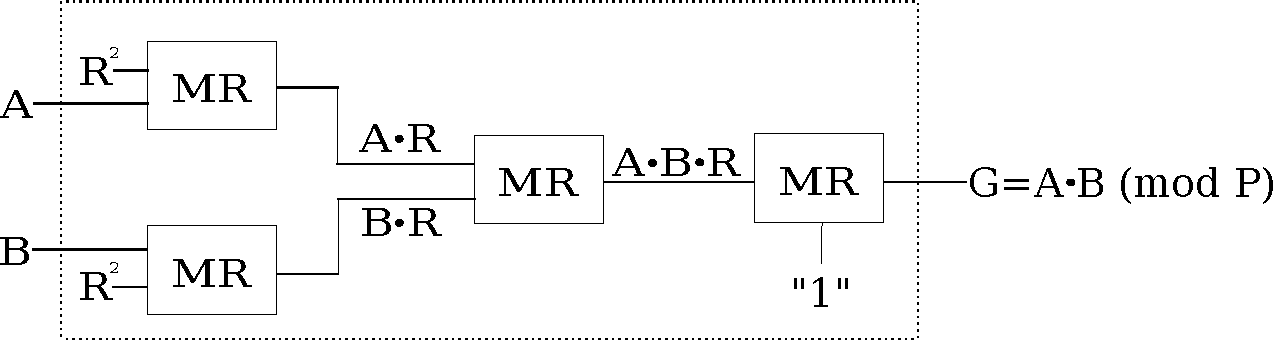
\includegraphics[scale=0.34]{new_mmcircuit-eps-converted-to}
%%   \caption{Montgomery multiplication.}
%%   \label{montfig}
%%   \end{figure}

Montgomery architectures~\cite{acar:1998},~\cite{wu:2002},
% \cite{Barrett:1987} 
~\cite{knezevic:2008} are considered more efficient than Mastrovito multipliers for exponentiation, 
as they do not require explicit reduction modulo $P(x)$ after each step.
%% ~\autoref{montfig} shows the structure of a Montgomery
%% multiplier. Each MR block computes $A\cdot B\cdot R^{-1}$, where $R$
%% is selected as a power of a base ($\alpha^{k}$) and $R^{-1}$ is the multiplicative 
%% inverse of $R$ in $\mathbb{F}_{2^k}$. As this operation cannot compute $A\cdot B$
%% directly, we need to pre-compute $A\cdot R$ and $B\cdot R$ as shown in the~\autoref{montfig}. 
%% We denote the leftmost
%% two blocks as Block A (upper) and B (lower), the middle block as Block
%% C and the output block as Block D.
% We have presented results for GBR
%on both \textit{flattened} and \textit{hierarchical} netlists of these
% multipliers.

~\autoref{masusmontspec} presents the results of our approach to debug
and rectification with the bugs placed in the Montgomery multiplier
with a Mastrovito multiplier circuit used as the specification. While
the approach~\cite{fujita:2015} finds a satisfying transformation
assignment which can be mapped to a library gate, our approach debugs
the circuit and finds a single fix rectification function. As shown in
the table, our approach shows improvement by several orders of
magnitude over \cite{fujita:2015}. 

%The comparison of bug placement reflects the complexity involved in
%debugging circuits where the bug lies in the deeper part ($NO$) of the
%topology.
It takes considerable amount of time for verification and
rectification check when the bug is close to the output. We are
working on further improving the experiments by employing better data
structures like  
ZBDDs~(\cite{minato:zbdd}), and devising better heuristics to perform
rectification check.
%We are also looking into efficient
%implementations for representing the partial remainder as a linear
%combination of an ideal during correction computation.
Due to several limitations w.r.t number of ring variables that can be
declared in SINGULAR, we have had to restrict our experiments within
64-bit data-path size.   

\section{Conclusions}

This paper has presented a fully automated debug approach for single fix rectification under RTTO$>$ based on \Grobner basis reductions and ideal
membership test. We presented a procedure to test for the existence of utilized the duality of varieties and ideals to check for the existence of single fix rectification at a given net. 
The experimental results demonstrate the efficacy of our approach for finite field arithmetic circuits where we achieve several orders of magnitude
improvement as compared to recent SAT-based approach. 
As part of our future work, we are working on improving the efficiency of our implementation to target higher bit-widths. We are also investigating how the current procedure can be extended to cover integer arithmetic circuits.
Further research also includes exploring the current approach for
the case of multi-fix rectification.  

\section{Conclusion}
\label{sec:conc}
This paper has presented a detailed theory and algorithm describing
the notion of Craig interpolants for a pair of polynomial ideals in
finite fields with no common zeros. The approach utilizes concepts
from computational algebraic geometry. Interpolants always exist in
this setting, and they correspond to the variety of an 
elimination ideal. In addition to defining the smallest and the largest
interpolants, techniques are described to compute them using Gr\"obner
basis concepts.  The total number of interpolants is also determined
by counting the number of points in the variety of (set) difference of
the largest and the smallest interpolants. Over the field $\F_2$, 
a technique is presented that can enumerate all possible interpolants. 
Given an interpolant, a heuristic algorithm is provided that 
returns a list of progressively larger interpolants, terminating in
the largest one. Experiments conducted demonstrate the validity of our
results. As part of future work, we are pursuing heuristic based 
methods to compute interpolants in a more controlled fashion and
classify them according to  their capability of abstraction. 


%%%%%%%%%%%%%%%%%%%% The bibliography %%%%%%%%%%%%%%%%%%%%%%%%%%%%
%\bibliographystyle{splncs03}
\bibliographystyle{IEEEtran}
%\bibliography{cf}
\bibliography{utkarsh,xiaojun,tim,logic,oldlogic,cnfsat,condrat_ms}
% \begin{thebibliography}{1}
% \bibliography{fmcad17}
% \end{thebibliography}

% \bibliography{utkarsh}
\newpage
\begin{center}
{\Large \bf Appendix: Omitted Proofs}
\end{center}


\par \noindent {\bf Proof of Theorem \ref{thm:smallest}.} 
\begin{proof}
Let $J_I \subseteq \Fq[C]$ be any another ideal-interpolant $\neq
J_S$. We show that $\Vc(J_S) \subseteq \Vc(J_I)$. For $\Vc(J_I)$
to be an interpolant it must satisfy 
\begin{align*}
\Vabc(J_A) \subseteq \Vabc(J_I)
\end{align*}
which is equivalent to 
\begin{align*}
I(\Vabc(J_A)) &\supseteq I(\Vabc(J_I)) \\
\implies J_A &\supseteq J_I  
\end{align*}
due to Theorem \ref{thm:strong-ns}.
%% as $J_I$ is radical so $I(\Vabc(J_I)) = J_I)$. 
As the generators of $J_I$ only contain polynomials in $C$-variables,
this relation also holds for the following
\begin{align*}
J_A \cap \Fq[C] &\supseteq J_I \\
\implies J_S &\supseteq J_I \\
\implies \Vc(J_S) &\subseteq \Vc(J_I).
\end{align*} 



\end{proof}

\par \noindent {\bf Proof of Theorem \ref{thm:large}.} 


\begin{proof} 
We first prove that the interpolant computed by
complementing $\Vc(J'_L)$  as $\Fq^C - \Vc(J'_L)$ is indeed a valid
interpolant. As $J'_L$ is the elimination ideal computed from $J_B$,
$\Vbc(J'_L) \supseteq \Vbc(J_B)$. This in turn implies that the
complement of $V(J'_L)$ cannot intersect with $V(J_B)$ at any
point. This proves condition 2 for $\Fq^C - \Vc(J'_L)$ to be a
valid interpolant.  

For condition 1, we need to prove that
\begin{align*}
\Vac(J_A) \subseteq \Fq^A \times (\Fq^C - \Vc(J'_L))
\end{align*}
This can be restated as
\begin{align*}
\Vac(J_A) \cap \Fq^A \times \Vc(J'_L) = \emptyset
\end{align*}
Let us assume (by contradiction) that there exists a common point 
$(\mathbf{a},\mathbf{c})$ in $\Vac(J_A)$ and $\Fq^A \times
V_C(J'_L)$. As the projection $Pr_B(\Vbc(J_B))$ on the
$C$-variables is equal to  the variety of the elimination ideal
$\Vc(J'_L)$, a point $(\mathbf{c}) \in \Vc(J'_L)$ can be  extended to
some point $(\mathbf{b},\mathbf{c})$ in $\Vbc(J_B)$. This implies that
the point $(\mathbf{a},\mathbf{b},\mathbf{c})$ is a common point in
$\Vabc(J_A)$ and $\Vabc(J_B)$, which is a contradiction to our initial
assumption. Therefore condition 1 of Def. \ref{def:int} is satisfied
too and $\Fq^C - \Vc(J'_L)$ is indeed an interpolant. 

\par \noindent Next we prove that $\Fq^C - \Vc(J'_L)$ is the largest
interpolant. Consider an arbitrary ideal-interpolant $J_I$. We want to
prove $\Vc(J_I) \subseteq \Fq^C - \Vc(J'_L)$, or equivalently to prove
$\Vc(J_I) \cap \Vc(J'_L) = \emptyset$. Let us assume (by contradiction) 
that there exists a common point $(\mathbf{c})$ in $\Vc(J_I)$ and
$\Vc(J'_L)$. As $J'_L$ is the elimination ideal of $J_B$, this point
can be extended to some point $(\mathbf{b},\mathbf{c})$  
in $\Vbc(J_B)$. This in turn implies that $(\mathbf{b},\mathbf{c})$ is
a common point in  $\Vbc(J_B)$ and $\Fq^B \times \Vc(J_I)$. This is a
contradiction as an interpolant cannot intersect with the variety of
$J_B$. Hence, $\Fq^C - \Vc(J'_L)$ is the largest interpolant and it
contains all other interpolants.

\end{proof}


\par \noindent {\bf Proof of Lemma \ref{noofinter}.} 
\begin{proof}
The smallest and the largest interpolants are $\Vc(J_S)$ and $\Vc(J_L)$,
respectively. The set difference $\Vc(J_L) - \Vc(J_S)$ is also a
variety of some ideal $J_D$, which can be computed as
$J_D=(J_L:J_S)$. By selecting different subsets of $\Vc(J_D)$ and
adding them to $\Vc(J_S)$, we can generate all the 
interpolants. Consider, 
\begin{align*}
\label{eqn:pwsetjd}
\binom{|\Vc(J_D)|}{0} + \binom{|\Vc(J_D)|}{1} + \cdots + \binom{|\Vc(J_D)|}{|\Vc(J_D)|} = 2^{|\Vc(J_D)|}
\end{align*}
where the term $\binom{|\Vc(J_D)|}{0}$ denotes that no point is selected from $\Vc(J_D)$ and results in 
$\Vc(J_S)$ as the ideal-interpolant. On the other hand, the term $\binom{|\Vc(J_D)|}{|\Vc(J_D)|}$ is equivalent 
to selecting  all the points from $\Vc(J_D)$ and results in $J_L$ as 
the ideal-interpolant. So the number of interpolants is equal to
$2^{|\Vc(J_D)|}$. Theorem \ref{thm:count} further tells us that the 
cardinality of a variety of an ideal is equal to the number of
standard monomials of that ideal, therefore, number of interpolants $=
2^{|SM(J_D)|}$.  

\end{proof}


\end{document}
